\documentclass[12pt,a4paper,onecolumn]{article}

%%%%%%%%%%%%%%%%%%%%%%%%%%%%%%%%%%%
%          				PACKAGES  				              %
%%%%%%%%%%%%%%%%%%%%%%%%%%%%%%%%%%%

\usepackage[colorlinks=true,linkcolor=black,urlcolor=blue,citecolor=blue]{hyperref}  % Necesario para usar \href y \url
\usepackage[margin=1in]{geometry}
\usepackage{authblk}
\usepackage[utf8]{inputenc}
\usepackage[spanish]{babel}
\usepackage{amsfonts}
%\usepackage{a4wide,graphicx,color}
\usepackage{graphicx}
\usepackage{amsmath}
\usepackage{amssymb}
\usepackage[table]{xcolor}
\usepackage{setspace}
\usepackage{booktabs}
\usepackage{dcolumn}
\usepackage{rotating}
\usepackage{color,soul}
\usepackage{threeparttable}
\usepackage[capposition=top]{floatrow}
\usepackage[labelsep=period]{caption}
\usepackage{array} % Para mejorar la alineación de las columnas
\usepackage{float}    % Permite usar [H] para colocar la tabla en una posición específica
\usepackage{booktabs} % Para mejorar la presentación de las tablas
\usepackage{subcaption}
\usepackage{lscape}
\usepackage{pdflscape}
\usepackage{multicol}
\usepackage[bottom]{footmisc}
\setlength\footnotemargin{5pt}
\usepackage{longtable} %for long tables
\usepackage{authblk}  % Agregar esto en el preámbulo
\usepackage{titling}
\usepackage{enumerate}
\usepackage{units}  %nicefraction
\usepackage{placeins}
\usepackage{booktabs,multirow}
%% BibTeX settings
\usepackage{natbib}
\bibliographystyle{apalike}
%\bibliographystyle{unsrtnat}
\bibpunct{(}{)}{,}{a}{,}{,}

%% NEEEEEWS

\usepackage{adjustbox} % Para ajustar el tamaño
\allowdisplaybreaks
\sloppy % ordena los elementos para evitar saltos de página

% Configuración de los enlaces
\usepackage{hyperref}
\hypersetup{
    colorlinks=true,     % Activar color en los enlaces
    linkcolor=black,     % Color de los enlaces de referencias y otras citas
    citecolor=black,     % Color de las citas
    filecolor=black,     % Color de los enlaces a archivos
    urlcolor=blue,       % Color de los enlaces URL
}

%% paragraph formatting
\renewcommand{\baselinestretch}{1}


% Defines columns for tables
\usepackage{array}
\newcolumntype{L}[1]{>{\raggedright\let\newline\\\arraybackslash\hspace{0pt}}m{#1}}
\newcolumntype{C}[1]{>{\centering\let\newline\\\arraybackslash\hspace{0pt}}m{#1}}
\newcolumntype{R}[1]{>{\raggedleft\let\newline\\\arraybackslash\hspace{0pt}}m{#1}}

\usepackage{comment} %to comment entire sections

\usepackage{xfrac} %sideways fractions


\usepackage{bbold} %for indicators
\usepackage{enumitem}

\setcounter{secnumdepth}{6}  %To get paragraphs referenced 

\usepackage{titlesec} %subsection smaller
\titleformat*{\subsection}{\normalsize \bfseries} %subsection smaller
%\usepackage[raggedright]{titlesec} % for sections does not hyphen words


\usepackage[colorlinks=true,linkcolor=black,urlcolor=blue,citecolor=blue]{hyperref}  %Load last
%% markup commands for code/software
\let\code=\texttt
\let\pkg=\textbf
\let\proglang=\textsf
\newcommand{\file}[1]{`\code{#1}'}
\newcommand{\email}[1]{\href{mailto:#1}{\normalfont\texttt{#1}}}
\urlstyle{same}

%%%%%%%%%%%%%%%%%%%%%%%%%%%%%%%%%%%%%%%%%%%%%%%%%%%%%%%%%%%
%     			TITLE, AUTHORS AND DATE    			  %
%%%%%%%%%%%%%%%%%%%%%%%%%%%%%%%%%%%%%%%%%%%%%%%%%%%%%%%%%%%
%% Title, authors and date

\title{Problem Set 1 - Grupo 10}

\author{
  Laura Buitrago Niño\thanks{\texttt{Facultad de Economía, Universidad de los Andes, Bogotá, Colombia. \textit{Email}: \href{mailto:la.buitragon1@uniandes.edu.co}{la.buitragon1@uniandes.edu.co}}}
  \quad
  María Camila Ortíz\thanks{\texttt{Facultad de Economía, Universidad de los Andes, Bogotá, Colombia. \textit{Email}: \href{mailto:mc.ortiza1@uniandes.edu.co}{mc.ortiza1@uniandes.edu.co}}}
  \quad
  Camilo Ramírez Arias\thanks{\texttt{Facultad de Economía, Universidad de los Andes, Bogotá, Colombia. \textit{Email}: \href{mailto:ca.ramirez10@uniandes.edu.co}{ca.ramirez10@uniandes.edu.co}}}
}

\date{\today}
\begin{document}
\maketitle
\thispagestyle{empty} % Leaves first page without page number

%%%%%%%%%%%%%%%%%%%%%%%%%%%%%%%%%%%
%          			  ABSTRACT       					      %
%%%%%%%%%%%%%%%%%%%%%%%%%%%%%%%%%%%

\begin{abstract}
Este estudio analiza la predicción de ingresos en Colombia para detectar posibles casos de evasión fiscal, utilizando datos de la GEIH 2018 para Bogotá, junto con el análisis teórico y empírico de la ecuación de Mincer. Se estiman regresiones lineales, incluyendo factores como la edad y el género, confirmando la relación en U invertida entre salario y edad y la brecha salarial de género. Los modelos predictivos con polinomios cuárticos e interacciones muestran mayor precisión, identificando casos de subdeclaración de ingresos. Los resultados destacan el potencial de estas herramientas para observar la fiscalización de ingresos por parte de las autoridades competentes.
\bigbreak
\textbf{Nota:} El repositorio relacionado a este documento se encuentra disponible en GitHub: \url{https://github.com/Laura-BN/ProblemSet1_G10}.
\end{abstract}

% Keywords and JEL Classification
\medskip

\begin{flushleft}
	{\bf Palabras clave:} Ecuación de Mincer, brecha salarial, predicción de ingresos, evasión fiscal, aprendizaje automático, economía laboral 				\\
	{\bf Clasificación JEL:} C53, J31, J30, H26
\end{flushleft}

% Ends title page and defines spacing for the rest of the document

%%%%%%%%%%%%%%%%%%%%%%%%%%%%%%%%%%%
%    DOCUMENT    		          %
%%%%%%%%%%%%%%%%%%%%%%%%%%%%%%%%%%%
\newpage
\section{Introducción} \label{sec:intro}

La creciente declaración de los ingresos individuales es crucial para el correcto y equitativo funcionamiento del sistema fiscal de los países. En este sentido, la evasión y fraude fiscal es un problema y desafío importante tanto en países con economías desarrolladas como con economías emergentes. Por ejemplo, en Estados Unidos para el 2001 la estimación general de la brecha fiscal bruta es de 345 mil millones de dólares, lo que representa el 16,3\% de la responsabilidad fiscal estimada \citep{slemrod2007}. La evasión o subdeclaración está impulsada por diversos factores tales como la falta de confianza en las autoridades fiscales, complejas normativas legales y la imposibilidad de supervisión efectiva \citep{alm2012}.
\bigbreak
Frente a esta situación, los modelos predictivos emergen como una herramienta útil para identificar patrones de comportamiento fiscal inusuales y predecir la probabilidad de evadir impuestos \citep{pomeranz2015}. Entonces, el uso de estas herramientas permite, por un lado, mejorar la precisión de las estimaciones de ingresos y, por otro, identificar posibles discrepancias que podrían indicar intentos de evasión fiscal \citep{torgler2007}. Esto podría contribuir a reducir los comportamientos evasivos y mejorar la eficiencia en la recaudación de impuestos, especialmente cuando se incluye en los análisis variables sociodemográficas tales como la edad, el sexo, el tipo de ocupación, la experiencia laboral, entre otras.
\bigbreak
Uno de los factores más relevantes en el análisis de los ingresos es la edad. \cite{mincer1974} planteó que los ingresos tienden a aumentar con la experiencia laboral hasta un punto máximo, tras el cual puede estabilizarse o disminuir debido a la pérdida de habilidades, disminución de la productividad y el envejecimiento. Su modelo estima las tasas de retorno de la edad, asociadas a la experiencia laboral, la capacitación en el trabajo, la educación y las diferencias de género \citep{Chiswick2006}. Por tanto, la relación salario y edad es crucial en la predicción de ingresos, puesto que los modelos pueden ajustar las estimaciones teniendo en cuenta las distintas fases de la vida laboral de las personas. De esta manera, se pueden detectar discrepancias entre los ingresos reportados y los esperados, especialmente en las franjas etarias con mayor riesgo de subdeclaración \citep{pomeranz2015}.
\bigbreak
La relación entre salario y sexo es otro aspecto trascendental que influye en los ingresos recibidos y reportados. La persistente brecha salarial de género ha sido ampliamente estudiada, arrojando como resultado que las mujeres obtienen menores ingresos que los hombres, incluso al controlar por educación, experiencia y otras variables \citep{blau2017}. En este sentido, es clave considerar este factor en los modelos predictivos debido a que podría afectar la precisión de las estimaciones de ingresos. De esta manera, se le incluye al modelo un componente que ayuda a detectar patrones de desigualdad salarial producto de los ingresos que deberían ser reportados entre hombres y mujeres, lo cual podría estar relacionado con la evasión fiscal \citep{goldin2014}.
\bigbreak
Los modelos predictivos que se basan en técnicas de aprendizaje estadístico pueden ser útiles para predecir los ingresos de los contribuyentes, lo cual ayuda a detectar posibles intentos de evasión fiscal. Al emplear variables como edad, sexo, número de hijos, nivel educativo, tipo de ocupación, industria, entre otros, permite estimar los ingresos esperados de un individuo y, con base en ello, identificar casos en los que los ingresos declarados no coinciden con lo esperado. Como señalan \cite{james2013}, las técnicas de aprendizaje automático, que incluyen tanto enfoques paramétricos como no paramétricos, ofrecen potentes herramientas para modelar la compleja relación entre las características sociodemográficas de los individuos y su comportamiento económico, lo que las hace bastante útiles para abordar la evasión fiscal.
\bigbreak
Precisamente, el presente documento realiza una aproximación a la predicción de ingresos de los individuos para abordar el problema de evasión fiscal. Para ello, se utilizan los datos de la Gran Encuesta Integrada de Hogares (GEIH) del DANE para el año 2018. Esta es una encuesta continua con cobertura nacional y es la fuente oficial de información estadística relacionada con mercado laboral, ingresos, pobreza monetaria y características sociodemográficas de la población residente en Colombia. Se clasifica a las personas según su fuerza de trabajo como población ocupada, desocupada o población fuera de la fuerza de trabajo. Por tanto, para el análisis se toman los datos de la población ocupada de 18 años en adelante, la cual nos brinda información acerca de ingresos laborales y otras rentas de las personas.
\bigbreak
El documento está construido de la siguiente manera. La sección 2 describe los datos, el proceso de depuración de estos y se presentan las principales estadísticas descriptivas. La selección de las variables predictoras del ingreso se basa en la ecuación de Mincer, que está fundamentada en la teoría del capital humano y en la amplia literatura empírica que ha validado su relevancia en la determinación de los ingresos.
\bigbreak
La sección 3 aborda el problema del perfil salarial por edad de la persona trabajadora. \cite{mincer1974} encontró que los salarios siguen una curva ascendente hasta alcanzar un máximo entre los 40 y 50 años. En este sentido, se encuentra que la relación ingreso-edad en Colombia sigue una tendencia en u invertida, con una edad pico del ingreso a los 42,09 años. A partir de dicho momento, en general, los trabajadores y trabajadoras colombianas presentan una reducción de sus ingresos.
\bigbreak
La sección 4 trata el problema de la brecha salarial de género utilizando la ecuación de Mincer ampliada con una variable dummy de género. La ecuación se extiende incorporando variables de capital humano, composición demográfica y características laborales para diferenciar el efecto de estos factores sobre la remuneración de hombres y mujeres. En general, los resultados evidencian la existencia de una brecha salarial de género económicamente relevante en favor de los hombres en Colombia. Asimismo, se observa que las mujeres alcanzan su pico salarial a los 44,84 años, es decir, casi dos años antes que los hombres con 46,65 años.
\bigbreak
La sección 5 evalúa el poder predictivo de los modelos con \textit{Cross-validation} y LOOCV. El MSE disminuye a medida que aumenta la complejidad del modelo, pero no necesariamente el modelo más complejo mejora el desempeño, indicando que más términos no siempre reducen el sesgo. El modelo con menor MSE contiene polinomios cuárticos e interacciones. La estimación de los errores de predicción en la muestra de prueba se concentran en 0, pero 2 \% de las observaciones son atípicas, con estimaciones superiores a los ingresos reportados, principalmente. Dado el autoreporte y el patrón sistemático de estos casos descrito en la sección, podría justificarse una revisión fiscal por parte de la DIAN.
\bigbreak
De forma general, en el presente documento se exploró la relación entre los ingresos individuales y diversas variables sociodemográficas, como la edad y el género, utilizando la ecuación de Mincer como base para la estimación de ingresos esperados para los trabajadores en Colombia. Se identificaron patrones consistentes con la literatura, como la curva en U invertida de los salarios y la persistente brecha salarial de género. Además, se evaluó el poder predictivo de distintos modelos, encontrando que aquellos con polinomios cuárticos e interacciones ofrecen mejores estimaciones. Finalmente, los resultados evidencian que el uso de modelos predictivos puede ser una herramienta útil para detectar posibles casos de evasión fiscal, permitiendo a las autoridades optimizar los procesos de fiscalización y mejorar la eficiencia en la recaudación de impuestos.


\section{Datos}\label{datos}

Los datos utilizados en este análisis provienen de la Gran Encuesta Integrada de Hogares (GEIH) de 2018, una fuente clave para la generación de indicadores del mercado laboral en Colombia. Esta encuesta tiene cobertura nacional y permite desagregar los resultados por zona urbana y rural, cinco grandes regiones (Atlántica, Oriental, Central, Pacífica y Bogotá), departamentos, 13 grandes ciudades con sus áreas metropolitanas y 11 ciudades intermedias. Sin embargo, para este estudio, se consideran únicamente los individuos residentes en Bogotá. Los datos contienen información a nivel individual sobre características demográficas básicas (ej. edad, sexo, género, nivel educativo), situación laboral (p. ej., formal, activo, ocupado, dependiente) y composición de ingresos, incluyendo información de las fuentes de ingresos principales y secundarias, así como percepciones por arrendamientos, pensiones y otros conceptos adicionales.
\bigbreak
Para la importación de los datos, fue necesario realizar un proceso de web \textit{scraping}, ya que la información no estaba disponible en un archivo descargable, sino distribuida en la página web del profesor Ignacio Barbieri\footnote{Los datos pueden encontrarse en el siguiente link: \url{https://ignaciomsarmiento.github.io/GEIH2018_sample}}. Los datos estaban segmentados en 10 \textit{chunks}, cada uno con aproximadamente 3,200 observaciones. Inicialmente, se intentó extraer las tablas directamente desde el HTML del sitio utilizando la librería $rvest$ en $R$. Sin embargo, las tablas no estaban contenidas en el código HTML estático de la página, indicativo de que los datos se cargaban de manera dinámica mediante peticiones de red. Para identificar la fuente de los datos, se inspeccionó la actividad de la red utilizando la pestaña $Network$ en las herramientas de desarrollo del navegador. Allí se observaron las solicitudes que el sitio web realizaba en segundo plano para recuperar la información. Tras analizar las peticiones, se identificaron los URL específicos desde donde la página obtenía cada fragmento de datos. Con esta información, se procedió a realizar la extracción en $R$ utilizando rvest, apuntando directamente a los URLs identificados en las solicitudes de red. 
\bigbreak
Una vez extraídos y agrupados los datos, la base inicial cuenta con 32,177 observaciones. Para este análisis, se considera únicamente la población ocupada puesto que son las personas que tienen información más completa .  En particular, los datos utilizados corresponden a personas ocupadas mayores de 18 años en Bogotá, con un total de 16,542 observaciones. 
\bigbreak
Con el fin de explicar el salario de los ocupados, se consideran variables como sexo, edad, formalidad laboral, cotización a pensión, tamaño de la firma, educación, nivel socioeconómico e ingresos (mensual y por hora). La selección sigue la ecuación de Mincer, basada en la teoría del capital humano y respaldada por evidencia empírica de Becker (1964) y Mincer (1957, 1958) \citep{Grossbard2006}. La educación y la experiencia reflejan la acumulación de habilidades que incrementan productividad y salarios. La edad y su término cuadrático capturan la relación no lineal con los ingresos (Varela et al., 2010). El género se incluye por su relación con brechas salariales y menor inversión en formación laboral de las mujeres (\cite{Chiswick2006}). Además, el tamaño de la empresa y la formalidad influyen en mejores remuneraciones (Brown y Medoff, 1989; Troske, 1999; Uribe and Ortiz, 2006).
\bigbreak
En este caso, la variable de ingreso, que suma el salario y los ingresos independientes, tiene 10.7 \% de valores faltantes ($NA$). El objetivo de este documento es predecir el ingreso por hora, por lo tanto, no se realiza imputación sobre estos valores faltantes para no distorsionar las relaciones subyacentes de este con otras variables. En tanto, se inició la construcción de la base final eliminando las observaciones con valores faltantes ($NA$) en la variable de ingreso, en la que quedaron finalmente 14,764 observaciones (ver cuadro \ref{diff_medias}). Por otro lado, se observa que la variable de ingresos, tanto por horas como mensuales, tiene varias observaciones en valores extremos (ver figuras \ref{boxplot_ing_horas} y \ref{boxplot_ing_mes}).  En la parte superior de la distribución (percentil 99) de ingresos por horas van desde \$ 62,349 pesos hasta los \$ 350,583 pesos por hora (148 obs); mientras que en el percentil 1 (143) va desde los \$ 0.47 a \$ 700 pesos. No obstante, estos valores (extremos) pueden ser reales y reflejar ocupaciones con ingresos significativamente altos/bajos. 

\begin{figure}[H] 
    \centering
    \caption{}\label{boxplot_ing_horas}
    \includegraphics[width=0.82\textwidth]{Graphs/box_plot_h.png} 
\begin{minipage}{15cm}
\small Nota: las líneas horizontales corresponden a los percentiles 99 (superior) y 1 (inferior) para cada variable
\end{minipage}
\end{figure}

En este documento, para la estimación de regresiones se emplean logaritmos del ingreso. El uso del logaritmo en regresiones (ej. ecuación de Mincer) tiene varias ventajas: facilita la linealización, reduce la varianza y permite una interpretación más clara. Además, captura la relación proporcional entre ingresos y otras variables, alineándose con el modelo de retornos del capital humano, donde la inversión en educación responde a expectativas de ganancia \citep{Lemieux2006}.
\bigbreak
En la figura \ref{Graphs/dif_medias_dicot} se observa que las variables que tienen una diferencia de medias estadísticamente significativa están relacionadas con el estado de formalidad del ocupado. En la muestra sin \textit{NA} en la variable ingreso, hay una mayor proporción de ocupados: en el sector formal, trabajando a tiempo completo, como obreros o empleados, y en firmas medianas o grandes (más de 50 empleados). En contraste, hay una menor representación de personas en el grupo etario de adultos mayores, trabajadores por cuenta propia o patrones/empleadores y que trabajen en microempresas. En cuanto a la variable de ingreso (por hora y mensual) las diferencias de medias no son estadísticamente significativas (cuadro \ref{diff_medias}) ya que se realiza el cálculo con las mismas observaciones en ambas muestras. 
\bigbreak
A pesar de que las diferencias son estadísticamente significativas, se procede con la estimación de diferentes regresiones a partir de la base sin $NA$ toda vez que no es deseable imputar una relación previa a la variable de interés (ingreso). 

\begin{figure}[H] 
    \centering
    \caption{}\label{Graphs/dif_medias_dicot}
    \includegraphics[width=1\textwidth]{Graphs/plot_dif_p.png} 
\begin{minipage}{15cm}
\small Nota: Se realizó una prueba t con un nivel de significancia del 5\%. Para todas las variables la prueba de diferencia de medias se realizó con $prop.test$. Para ver los valores específicos ver el cuadro 
\ref{diff_medias}. 
\end{minipage}
\end{figure}

A continuación, la distribución de las variables de la base final (cuadro \ref{diff_medias}). Respecto a la condición laboral, 60.2\% de los individuos tienen empleos formales, mientras que el 39.8\% están en la informalidad. Del total de ocupados, 47.3\% son mujeres, y la experiencia laboral promedio (en la empresa en la que trabaja) es de 5.3 años. El 68.3\% de ocupados trabaja a tiempo completo, la mayoría trabaja en una microempresa (49.6\%), seguido por empresa mediana o grande (37.6\%) y pequeña empresa (12.8\%). En cuanto al tipo de ocupación, la mayor parte son obreros o empleados (63.2\%), seguidos de cuenta propia (29.7\%) y empleados domésticos (3.8\%). Los patrones o empleadores representan el 3.2\% de la muestra.
\bigbreak
Casi la mitad de los ocupados (49,2 \%) tienen entre 29 y 50 años (adulto), 27,0 \% son jóvenes (18-28 años) y 23.8 \% tienen más de 50 años (adultos mayores). En la distribución socioeconómica gran parte de los ocupados son estrato 2 o 3 (78.6 \%); 10.9 \% son estrato 1; 6.5 \% son estrato 4 y los ocupados de estrato 5 y 6 representan 4 \% 
\bigbreak
Estrato socioeconómico: La mayoría pertenece a estratos 2 (42.9\%) y 3 (35.7\%), mientras que los estratos altos (5 y 6) tienen una menor representación (1.7\% y 2.3\%, respectivamente). Finalmente, el ingreso mensual promedio es de \$1,617,550.5 pesos (se: \$20,009.7) y el ingreso por hora es de \$8,541.9 pesos (se: \$114.1). En general, la dispersión de las variables en la muestra sin valores faltantes en ingreso es baja, como lo indican los errores estándar relativamente pequeños en todas las categorías.

\begin{table}[ht]
\centering
\caption{Diferencia de medias de variables entre muestras con y sin $NA$ en ingreso - Bogotá 2018}\label{diff_medias}
\resizebox{\textwidth}{!}{ 
\begin{tabular}{lrrrrrrl}
  \hline
Variable & Media\_1 (con NA) & se\_1 & Media\_2 (sin NA) & se\_2 & Dif & p\_valor & Significancia \\ 
  \hline
formal & 58.7 & 0.4 & 60.2 & 0.4 & -1.6 & 0.0 & *** \\ 
  informal & 41.3 & 0.4 & 39.8 & 0.4 & 1.6 & 0.0 & *** \\ 
  Mujer & 47.0 & 0.4 & 47.3 & 0.4 & -0.3 & 0.6 &  \\ 
  Experiencia & 5.4 & 0.2 & 5.3 & 0.2 & 0.1 & 0.8 &  \\ 
  Full\_time & 67.1 & 0.4 & 68.3 & 0.4 & -1.2 & 0.0 & *** \\ 
  Joven (18-28 años) & 26.1 & 0.3 & 27.0 & 0.4 & -0.8 & 0.1 &  \\ 
  Adulto (29-50 años) & 48.5 & 0.4 & 49.2 & 0.4 & -0.7 & 0.2 &  \\ 
  Adulto\_m (más de 50 años) & 25.3 & 0.3 & 23.8 & 0.4 & 1.5 & 0.0 & *** \\ 
  Estrato\_1 & 10.7 & 0.2 & 10.9 & 0.3 & -0.2 & 0.6 &  \\ 
  Estrato\_2 & 41.8 & 0.4 & 42.9 & 0.4 & -1.1 & 0.1 &  \\ 
  Estrato\_3 & 36.2 & 0.4 & 35.7 & 0.4 & 0.5 & 0.4 &  \\ 
  Estrato\_4 & 6.8 & 0.2 & 6.5 & 0.2 & 0.3 & 0.3 &  \\ 
  Estrato\_5 & 1.9 & 0.1 & 1.7 & 0.1 & 0.2 & 0.2 &  \\ 
  Estrato\_6 & 2.6 & 0.1 & 2.3 & 0.1 & 0.3 & 0.1 &  \\ 
  Tam\_firma\_Micro (0-10 ocup) & 51.6 & 0.4 & 49.6 & 0.4 & 2.0 & 0.0 & *** \\ 
  Tam\_firma\_Pequeña (10-50 ocup) & 12.4 & 0.3 & 12.8 & 0.3 & -0.4 & 0.3 &  \\ 
  Tam\_firma\_Mediana\_grande (más de 50 ocup) & 36.0 & 0.4 & 37.6 & 0.4 & -1.6 & 0.0 & *** \\ 
  Ocupacion\_cat\_Obreros\_empleados & 60.3 & 0.4 & 63.2 & 0.4 & -2.9 & 0.0 & *** \\ 
  Ocupacion\_cat\_Emp\_domésticos & 3.5 & 0.1 & 3.8 & 0.2 & -0.3 & 0.1 &  \\ 
  Ocupacion\_cat\_Cuenta\_propia & 30.9 & 0.4 & 29.7 & 0.4 & 1.1 & 0.0 & *** \\ 
  Ocupacion\_cat\_Patron\_empleador & 3.8 & 0.1 & 3.2 & 0.1 & 0.6 & 0.0 & *** \\ 
  Ocupacion\_cat\_Jornalero\_peon & 0.0 & 0.0 & 0.0 & 0.0 & -0.0 & 1.0 &  \\ 
  Ocupacion\_cat\_Otro & 0.1 & 0.0 & 0.1 & 0.0 & 0.0 & 1.0 &  \\ 
  y\_total\_m & 1,617,550.5 & 20,009.7 & 1,617,550.5 & 20,009.7 & 0.0 & 1.0 &  \\ 
  y\_total\_m\_ha & 8541.9 & 114.1 & 8541.9 & 114.1 & 0.0 & 1.0 &  \\ 
\hline
\hline
Observaciones & 16,542  & 14,764 & &  & & &  \\ 
\hline

\end{tabular}
}
\begin{minipage}{16cm}
\tiny Nota: Se realizó una prueba t con un nivel de significancia del 5\%. Para todas las variables, a excepción de $y\_total\_m$ y $y\_total\_m\_ha$ (ingreso mensual y por hora), la prueba de diferencia de medias se realizó con $prop.test$, en las dos restantes se usó $t.test$ de $R$. La columna \textit{Media\_2 (sin NA)} corresponde a los datos de la base sin valores faltantes de las variables de ingreso antes mencionadas. 
\end{minipage}
\end{table}

\bigbreak

\section{Perfil salarial por edad}

Una gran cantidad de evidencia en economía laboral sugiere que el perfil salarial por edad del trabajador típico tiene una trayectoria predecible: los salarios tienden a ser bajos cuando el trabajador es joven; aumentan a medida que el trabajador envejece, alcanzando un máximo alrededor de los 50 años; y la tasa salarial tiende a permanecer estable o disminuir levemente después de los 50 años".
\bigbreak 
En esta subsección vamos a estimar el perfil salarial por edad para los individuos en esta muestra:

\begin{equation}
    \log(w) = \beta_0 + \beta_1 \text{Age} + \beta_2 \text{Age}^2 + u
    \label{eq:age_wage}
\end{equation}

\bigbreak
donde donde $log(w)$ es el logaritmo natural del ingreso del individuo, $Edad$ es la edad del individuo y $u$ es el termino de error.

\begin{comment}
  {\color{red}
Al presentar y discutir sus resultados, incluya:
\begin{itemize}
    \item Una tabla de regresión.
    \item Una interpretación de los coeficientes y su significancia.
    \item Una discusión del ajuste del modelo en la muestra
    \item Un gráfico del perfil salarial por edad estimado implícito en la ecuación anterior.
    \item Incluyendo un análisis de la ``edad pico'' con sus respectivos intervalos de confianza.
    \item[](Nota: Use bootstrap para construir los intervalos de confianza).
\end{itemize}}  
\end{comment}

\subsection{Perfil salarial por edad del trabajador}

La relación entre la edad de los trabajadores y su perfil salarial ha revelado que existen patrones predecibles en la evolución de los salarios a lo largo de la vida laboral. Según la teoría del capital humano de \cite{becker1964}, los salarios inicialmente son bajos porque las personas jóvenes tienen baja experiencia y menor productividad. A medida que las personas aumentan su experticia y habilidades, su valor en el mercado laboral aumenta, lo que conlleva a un aumento salarial progresivo.
\bigbreak
En este sentido, \cite{mincer1974} encontró que los salarios siguen una curva ascendente hasta alcanzar un máximo entre los 40 y 50 años. Ello se explica porque en la mediana edad las personas tienen su mayor nivel de experiencia, mejores cualidades y pueden acceder a puestos estables, de mayor responsabilidad y con mejores remuneraciones. A partir de ese punto, los salarios tienden a estabilizarse o incluso a disminuir debido a la obsolescencia de habilidades o la menor demanda de trabajo en ciertas industrias \citep{juhn1993}.
\bigbreak
Precisamente, a continuación se analizará el perfil salarial por edad para los individuos de la muestra para el año 2018 de la Gran Encuesta Integrada de Hogares (GEIH) del DANE, cuyos datos se describieron en la sección anterior. Para ello, se estima la ecuación \ref{eq:age_wage} estableciendo la relación del ingreso con la edad y con un polinomio grado 2, cuyos resultados se pueden observar en la columna (1) y (2) del cuadro \ref{tab:regresion_ec1}, respectivamente.
\bigbreak
En primera instancia, tal como se observa en la columna (1) no se evidencia una relación entre el ingreso y el salario, esto quiere decir, que no existe una relación lineal entre la edad y el ingreso laboral de las personas. Ello precisamente se evidencia en la columna (2) en la que se aborda esta problemática con un polimonio de grado 2, tal como está explícito en la ecuación \ref{eq:age_wage}.
\bigbreak
La columna (2) del cuadro \ref{tab:regresion_ec1} muestran que el coeficiente de la edad es positivo y estadísticamente significativo al nivel de 1\%. Esto sugiere que, el aumento en una unidad de la edad se asocia a un aumento de aproximadamente 5\% en el salario. Ahora bien, el coeficiente negativo de la edad al cuadrado y estadísticamente significativo al nivel de 1\%, indica que el efecto de la edad en los salarios no es lineal. Así pues, a medida que la edad aumenta, el salario continua aumentando, pero a una tasa decreciente. 
\bigbreak

% Tabla resultados ecuación 1: log(w) = edad + edad^2
\begin{table}[htbp] \centering 
  \caption{Resultados estimación perfil salarial por edad} 
  \label{tab:regresion_ec1} 
\begin{tabular}{@{\extracolsep{5pt}}lcc} 
\\[-1.8ex]\hline 
\hline \\[-1.8ex] 
 & \multicolumn{2}{c}{\textit{Variable dependiente:}} \\ 
\cline{2-3} 
\\[-1.8ex] & \multicolumn{2}{c}{Log(ingreso)} \\ 
\\[-1.8ex] & (1) & (2)\\ 
\hline \\[-1.8ex] 
 Edad & 0.0001 & 0.055$^{***}$ \\ 
  & (0.001) & (0.003) \\ 
  & & \\ 
 Edad al cuadrado &  & $-$0.001$^{***}$ \\ 
  &  & (0.00004) \\ 
  & & \\ 
 Constante & 8.622$^{***}$ & 7.578$^{***}$ \\ 
  & (0.021) & (0.060) \\ 
  & & \\ 
\hline \\[-1.8ex] 
Observaciones & 14,764 & 14,764 \\ 
R$^{2}$ & 0.00000 & 0.023 \\ 
R$^{2}$ ajustado & $-$0.0001 & 0.023 \\ 
Error estd. residual & 0.833 (df = 14762) & 0.823 (df = 14761) \\ 
F-estadístico & 0.014 (df = 1; 14762) & 172.957$^{***}$ (df = 2; 14761) \\ 
\hline 
\hline \\[-1.8ex] 
\end{tabular} 
\begin{minipage}{14cm}
\small Notas: La variable de ingreso corresponde al logaritmo natural del ingreso por hora de las personas ocupadas asalariadas e independientes. $^{*}$p$<$0.1; $^{**}$p$<$0.05; $^{***}$p$<$0.01.
\end{minipage}
\end{table}
% Fin tabla

Ahora bien, es importante analizar el grado en el cual el modelo se ajusta a los datos. La calidad de la regresión lineal es típicamente evaluada usando dos cantidades relacionadas: el \textit{error estándar residual (RSE)} y el estadístico \( R^2 \) \citep{james2013}. 
\bigbreak
El RSE es una estimación de la desviación estándar de $u$, por lo que representa la cantidad promedio en que la respuesta se desvía de la verdadera línea de regresión \citep{james2013}. En otras palabras, es una medida de la falta de ajuste del modelo a los datos. Tal como se muestra en la columna (2), el error estándar de las estimaciones de la ecuación \ref{eq:age_wage} es 0.823, lo que significa que el modelo no tiene un buen ajuste a los datos teniendo en cuenta que el rango  del logaritmo del ingreso por hora trabajada no es grande (-0.75,12.77). Así pues, este error estándar sugiere que, aunque el modelo no es completamente ineficaz, las predicciones pueden ser imprecisas.
\bigbreak
Ahora bien, el RSE proporciona una medida de la falta de ajuste del modelo a los datos, medido en unidades de la variable dependiente. Por tanto, no siempre es claro que constituye una buena medida de este. De esta manera, el \( R^2 \) brinda una medida alternativa de ajuste con una ventaja de interpretativa en tanto que va de 0 a 1 \citep{james2013}. Este mide la proporción de la variabilidad de la variable dependiente que es explicada por las variables independientes en el modelo de regresión.
\bigbreak
Tomando el \( R^2 ajustado \), ya que tiene en cuenta el número de predictores en el modelo, en la columna (2) de la ecuación \ref{eq:age_wage} observamos que este estadístico tiene un valor de 0.023. Esto nos indica que solo el 2.3\% de la variabilidad en los logaritmos de los ingresos por hora trabajada son explicados por el modelo, es decir, por las variables de $Edad$ y $Edad\textsuperscript{2}$. Esto sugiere que el modelo tiene un ajuste muy bajo, por lo cual no es eficaz en explicar el ingreso de los individuos, ya que existe una gran cantidad de variabilidad que no se explica por las variables incluidas. 
\bigbreak
Así pues, el ajuste del modelo a los datos evaluado por el $RSE$ y el  \( R^2 ajustado \), nos indican que la $Edad$ y la $Edad\textsuperscript{2}$ probablemente no son los únicos aspectos que afectan el salario. Factores tales como la educación, el sexo, la experiencia laboral, la industria en la que trabaja, entre otros, pueden afectar el ingreso laboral de las personas, lo cual se abordará en la sección 4. Ahora bien, si bien es cierto que existen otras variables relacionadas no incluidas, el valor de 172.9 del \textit{estadístico F} nos sugiere que efectivamente existe una relación entre el ingreso por hora trabajada y la edad de las personas.
\bigbreak
Ahora bien, los resultados de los coeficientes de la estimación de la ecuación \ref{eq:age_wage} son consistentes con la teoría de que los salarios aumentan hasta un punto máximo entre los 40 y 50 años \citep{mincer1974}. En este sentido, a continuación abordamos la relación entre la edad y el ingreso de las personas.


\subsection{Edad pico}

El concepto de ``$edad$ $pico$'' en el perfil salarial hace referencia a la edad en la cual los salarios alcanzan su nivel máximo antes de comenzar a disminuir. \cite{mincer1974} aporta una explicación fundamental sobre cómo la experiencia y la educación afectan los salarios a lo largo de la vida laboral, identificando que los salarios tienden a alcanzar un pico alrededor de los 40-50 años antes de comenzar a declinar debido a factores como la obsolescencia de habilidades y la disminución de la productividad marginal.
\bigbreak
Ahora bien, el perfil salarial de los trabajadores no es homogéneo 
 ya que depende de la trayectoria laboral de los individuos. Los ingresos laborales alcanzan un pico a medida que los trabajadores ganan experiencia y acumulan habilidades. No obstante, existe un punto en el que la curva de ganancias comienza a decrecer debido a la reducción en los rendimientos marginales de la experiencia por factores tales como la depreciación de las habilidades y el envejecimiento físico de la población trabajadora \citep{willis1986}.
\bigbreak
 La $edad$ $pico$ puede variar dependiendo del tipo de industria y el impacto de los avances tecnológicos \citep{acemoglu2018}. Por ejemplo, la automatización y la digitalización están cambiando las trayectorias salariales de los trabajadores, de modo que en ciertos sectores, como la tecnología o las ciencias, los salarios pueden seguir siendo altos durante más tiempo debido a la actualización constante de habilidades \citep{brynjolfsson2014}. En ciertas industrias, los trabajadores en adultez mayor tienen la oportunidad de mantener altos niveles salariales gracias a su experiencia y conocimientos acumulados, incluso cuando las tendencias salariales en general indican un decrecimiento con la edad \citep{autor2020}.
\bigbreak
Ahora bien, una comprobación visual de las teorías relacionadas con la $edad$ $pico$, se puede observar en la figura \ref{fig:age_wage_profile}, la cual muestra la relación de edad-ingreso con base en las estimaciones de la ecuación \ref{eq:age_wage}. Tal como se observa, el ingreso de las personas aumenta hasta alcanzar su máximo hacia los 40 años. Luego de ello, decrece a medida que la persona aumenta su edad, llegando a partir de los 60 años a niveles inferiores que los del inicio de la actividad laboral en los 18 años.
\bigbreak
\begin{figure}[H]
    \centering
    \includegraphics[width=0.7\linewidth]{Graphs/age_wage_profile.png}
    \caption{Perfil estimado de ingresos por edad}
    \label{fig:age_wage_profile}
    \vspace{0.2cm} % Espacio pequeño entre la tabla y la nota
    \begin{minipage}{0.9\textwidth}  
    \footnotesize \scriptsize { \textit{Notas:} La estimación de la relación de ingresos y edad se realizó para la población mayor a 18 años con base en la ecuación \ref{eq:age_wage}. La zona sombreada corresponde al intervalo de confianza al 95\%.Los valores de ingreso por hora trabajada están en pesos colombianos de 2018.}
    \end{minipage}
\end{figure}

\bigbreak
Ahora bien, la $edad$ $pico$ es el momento en que el salario de una persona alcanza su máximo. Para estimarla, tomamos la derivada de la ecuación \ref{eq:age_wage} con respecto a $Age$:
\[
\frac{\partial\log(w)}{\partial\text{Age}} = \beta_1 + 2 \beta_2 \cdot \text{Age}
\]
\bigbreak
Para encontrar el valor de la edad en la que el salario es máximo, igualamos la derivada a cero:
\[
\beta_1 + 2 \beta_2 \cdot \text{Age} = 0
\]

Despejamos $Age$ de la ecuación:

\[
2 \beta_2 \cdot \text{Age} = -\beta_1
\]

\[
\text{Age} = -\frac{\beta_1}{2 \beta_2}
\]
Por tanto, la $edad$ $pico$, es decir, la edad en la que el salario alcanza su máximo, está dada por:

\begin{equation}
   Age_{peak} = -\frac{\beta_1}{2 \beta_2}
    \label{eq:age_peak}
\end{equation}
\bigbreak
Con base en la estimación por $bootstrap$ de la ecuación \ref{eq:age_wage}, se obtiene que la edad pico de la población ocupada en 2018 en Colombia fue de 42.09 años, tal como se muestra en el cuadro \ref{tab:edad_pico_estimada}. La incertidumbre asociada a esta estimación es de $\pm\ $0.43 años, lo cual significa que si repetimos el proceso de $bootstrap$ $n$ veces para estimar la edad a partir de los diferentes remuestreos de los datos, las estimaciones de la $edad$ $pico$ fluctuarían dentro de un rango de aproximadamente 42.09 $\pm\ $0.43 años. De esta manera, la $edad$ $pico$ estimada es bastante precisa ya que el error estándar es relativamente pequeño en comparación con el valor de la estimación.

% Tabla edades pico estimadas bootstrap
\begin{table}[ht]
\caption{$Edad$ $pico$ estimada}
\label{tab:edad_pico_estimada} 
\centering
\begin{tabular}{lr}
  \hline
  Concepto & Valor \\ 
  \hline
Edad pico estimada & 42.09 \\ 
Error estándar & 0.43 \\ 
Límite superior  & 43.02 \\ 
Límite inferior & 41.29 \\ 
   \hline
\end{tabular}
\vspace{0.5cm}
\begin{minipage}{0.7\textwidth}  
\footnotesize \scriptsize { \textit{Nota}: La edad pico se estimó como el punto máximo de la curva salario-edad. El valor de la edad pico, el error estándar y el intervalo de confianza al 95\% se construyen usando $bootstrap$ con 10.000 iteraciones de remuestreo con base en la ecuacion \ref{eq:age_wage}}
\end{minipage}
\end{table}
Ahora bien, la figura \ref{tab:intervalo_edad_pico} muestra la distribución de las estimaciones por $bootstrap$, así como su respectivo intervalo de confianza. En la parte izquierda se evidencia que la distribución de estas se encuentra concentrada alrededor de la $edad$ $pico$, tal como también puede evidenciarse en la parte derecha del gráfico. Adicionalmente, se espera que el valor estimado se encuentre en el rango [41.29,43.02] con un 95 \% de confianza. 

% Gráfico edad pico
\begin{figure}[H]
    \centering
    \includegraphics[width=0.7\linewidth]{Graphs/age_wage_box-plot.png}
    \caption{Distribución de la $edad$ $pico$ estimada}
    \label{tab:intervalo_edad_pico}
    %\vspace{0.2cm} % Espacio pequeño entre la tabla y la nota
    \begin{minipage}{0.8\textwidth}  
    \footnotesize \scriptsize { \textit{Notas:} $Izquierda$: Un histograma de las estimaciones de la $edad$ $pico$ obtenidas al genererar 10.000 simulaciones del conjunto de datos de la verdadera población. $Derecha$: Boxplot con base en las estimaciones de la $edad pico$ mostradas en la izquierda, incluyendo un intervalo de confianza de la $edad pico$ al 95\% construido usando $bootstrap$ con 10.000 iteraciones de remuestreo con base en la ecuación \ref{eq:age_wage}. En ambos paneles la línea roja indica el valor máximo estimado de la $edad pico$.}
    \end{minipage}
\end{figure}
\bigbreak
Por tanto, tal como enunciaron \cite{mincer1974} y \cite{willis1986} en sus trabajos, en el caso de la población ocupada colombiana encontramos que la $edad$ $pico$ de su ingreso está en los 42.09 años, para luego empezar a decrecer. Sin embargo, es importante tener en cuenta que aunque estos resultados son estimados para el agregado de las personas trabajadoras, la máxima relación de edad-ingreso puede variar a partir de particularidades propias de cada industria y el impacto de los avances tecnológicos \citep{acemoglu2018}. En este mismo sentido, puede existir un comportamiento diferenciado entre hombres y mujeres, lo cual se aborda en la siguiente sección.  
\bigbreak

% Tabla resultados edad pico
%\begin{table}[ht]
%\centering 
%\caption{Estimaciones de $edad$ $pico$}
%\label{tab:intervalo_edad_pico} 
%\begin{tabular}{rlr}
%  \hline
% & Concepto & Edad \\ 
%  \hline
%    1 & Edad pico estimada & 42.09 \\ 
%    2 & Límite inferior & 41.29 \\ 
%    3 & Límite superior & 43.02 \\ 
%   \hline
%\end{tabular}
%\vspace{0.5cm} % Espacio pequeño entre la tabla y la nota
%\begin{minipage}{0.8\textwidth}  
%\footnotesize \scriptsize { \textit{Notas:} El intervalo de confianza de la $edad$ $pico$ al 95\% se construye usando $bootstrap$ con 10.000 iteraciones de remuestreo con base en la ecuacion \ref{eq:age_wage}.}
%\end{minipage}
%\end{table}


\section{La brecha salarial de género}
Existe una amplia literatura que analiza la brecha salarial de género utilizando la ecuación de Mincer ampliada con una variable \textit{dummy} de género. En el presente análisis, se emplea esta especificación para analizar las diferencias salariales entre hombres y mujeres. \\
\bigbreak
La ecuación se extiende incorporando dimensiones de capital humano, composición demográfica y características laborales, con el objetivo de identificar la brecha salarial de género separándola de las diferencias en ingresos relacionadas con características laborales y personales. Es fundamental reconocer que la ecuación de Mincer enfrenta diversos problemas econométricos ampliamente reconocidos en la literatura, tales como la omisión de variables, la selectividad muestral, los regresores endógenos y la multicolinealidad \citep{polachek2007}. Por esta razón, aunque varios factores han demostrado influir en los ingresos, no se han considerado ciertas variables que podrían estar relacionadas con características no observables o que podrían estar altamente correlacionadas con otros regresores. Un ejemplo de ello son el estado civil y el número de hijos, cuya inclusión podría generar sesgo, ya que es probable que estas variables sean endógenas con respecto a las decisiones laborales de las mujeres. \\

De este modo, se estima la brecha salarial condicional mediante la siguiente especificación:
\begin{align}
\label{eq:mincer}
\log(w_{i}) = & \, \beta_0 + \beta_1  \text{Female}_i + \beta_2 \text{Age}_i + \beta_3  \text{Age}^2_i + \beta_4  \text{Educ}_i \nonumber \\
& + \beta_5  \text{Seniority}_i   + \beta_6  \text{Seniority}^2_i + \beta_7 \text{FirmSize}_i \nonumber \\ 
& + \beta_8 \text{Fulltime}_i + \beta_9 \text{Formal}_i  +  \beta_{10} \text{JobCategory}_i  +  \epsilon_i
\end{align}


El ingreso por hora \textit{w} de cada individuo $i$ está modelado como una función de diversas variables. La selección de cada una de las variables incluidas como determinantes del salario se han basado en la evidencia registrada en la literatura. La variable \textit{Female} es dicotómica y toma el valor de 1 si el individuo es mujer y 0 en caso contrario, este es el coeficiente que permite capturar la brecha de genero salarial. La variable \textit{Age} representa la edad del individuo, y $Age^2$ es su cuadrado, incluido para capturar la típica relación en forma de ``curva en U invertida'' entre edad y salario registrada en la literatura \citep{varela2010}. Esta relación sugiere que los salarios tienden a aumentar conforme una persona gana experiencia laboral, para luego estabilizarse o incluso disminuir a medida que se acerca a la jubilación. \\

De acuerdo con la Teoría del Capital Humano \citep{becker1964}, la educación es vista como una inversión que mejora la productividad de las personas, lo que, a su vez, aumenta su capacidad para generar ingresos, por lo cual se incluye la variable categórica \textit{Educ} que se define en las siguientes categorías: sin educación completa (aquellos que no han terminado la primaria o la secundaria), primaria completa, secundaria completa y educación superior completa. Es importante reconocer, que este modelo puede estar sujeto a un problema de variable omitida, ya que no se controla por las habilidades no observables que también influyen en la productividad y los ingresos. Las habilidades pueden estar correlacionadas con el nivel educativo y afectar tanto el rendimiento educativo como los ingresos, lo que podría sesgar los resultados. \\

Por otro lado, la experiencia es un factor de capital humano con efectos similares a la edad y la literatura suele incluirla dentro de la ecuación de Mincer,  dado que refleja la acumulación de habilidades adquiridas post-escolarización, lo que impacta directamente en la productividad y los ingresos.  Aunque la edad se usa comúnmente como proxy de experiencia, omitir la experiencia podrían generar resultados sesgados. La experiencia y la escolaridad están negativamente correlacionadas (es decir, las personas con más escolaridad a menudo tienen menos años de experiencia laboral a la misma edad), y tanto la escolaridad como la experiencia están positivamente correlacionadas con los ingresos. Por lo tanto, omitir la experiencia podría resultar en una subestimación del efecto de la escolaridad sobre los ingresos \citep{patrinos2016}.  \\

Aunque la información disponible se refiere únicamente a la experiencia en la ocupación principal y no a la experiencia laboral total acumulada, esta puede ser una aproximación válida de la experiencia total, especialmente si los individuos han tenido trayectorias laborales estables. El promedio de 60 meses de experiencia (5 años) indica una trayectoria laboral suficiente para generar incrementos significativos en los ingresos, particularmente en los primeros años de desempeño en una ocupación. No obstante, al igual que con la experiencia total, es razonable esperar rendimientos decrecientes: los mayores aumentos en ingresos suelen ocurrir al inicio, cuando se consolidan las habilidades, mientras que con el tiempo el crecimiento salarial tiende a estabilizarse o incluso a disminuir. Por lo cual, para capturar esta dinámica no lineal, se incluye el término cuadrático de la experiencia. \\

De igual manera, incorporar el tamaño de la empresa en la ecuación de Mincer es relevante porque las empresas grandes suelen pagar salarios más altos \citep{brown1989, troske1999}. La variable \textit{Firmsize} es categórica y clasifica a las empresas en tres tamaños: microempresa, pequeña empresa y mediana-grande empresa. En la misma línea, según el enfoque estructuralista, un mercado laboral formal sugiere un mejor pago, dado que cuenta con mejores condiciones laborales y mayor calidad de sus trabajadores \citep{uribe2006}. Por lo cual, \textit{Formal} es una variable dicotómica que toma el valor de 1 si el individuo tiene un empleo formal y 0 en caso contrario. \\

Distintos tipos de ocupaciones pagan salarios diferentes, incluso para trabajadores con características similares. Si no se controla por el tipo de ocupación, parte de la brecha salarial observada podría deberse a que hombres y mujeres están sobrerrepresentados en industrias con diferentes niveles de remuneración. Este fenómeno no necesariamente refleja discriminación de género, sino que puede estar relacionado con las elecciones laborales que los hombres y las mujeres hacen. Estudios como el de \cite{tenjo2005} indican que las mujeres, debido a sus responsabilidades de trabajo doméstico y cuidado infantil, tienden a elegir ocupaciones que ofrecen horarios más flexibles o menos demandantes. Según \cite{arriagada1998}, las mujeres pueden estar sobre-representadas en sectores de baja productividad. Por lo cual, se incluye la variable $JobCategory$ que identifica a los trabajadores en las categorias de: Directores y Gerentes, Profesionales, Científicos e Intelectuales, Técnicos, Profesionales Nivel Medio, Apoyo Administrativo, Trabajadores de Servicios, Comercios y Mercados, Agricultores y Trabajadores Calificados Agro, Oficiales, Operarios, Artesanos y Oficios Relacionados, Operadores de Instalaciones, Máquinas y Ensambladores, y Ocupaciones Elementales. \\

Finalmente, el término de error $\epsilon_i$ representa un componente aleatorio que captura las perturbaciones individuales y se asume que sigue una distribución normal. \\

Empezamos estimando la brecha salarial no condicional mediante una regresión del logaritmo del salario sobre una variable indicadora que toma el valor de 1 si el individuo es mujer. Sin embargo, esta estimación puede estar sesgada, ya que no considera diferencias en la composición de la fuerza laboral entre hombres y mujeres, lo que impide identificar si la brecha observada se debe a disparidades en características productivas o a discriminación salarial. Para abordar este problema y evaluar si individuos con características similares reciben salarios similares, se estima la brecha salarial condicional a través de la ecuación (\ref{eq:mincer}), utilizando el teorema de Frisch-Waugh-Lovell para obtener el coeficiente asociado a la variable $Female$. Finalmente, se vuelve a estimar la brecha condicional aplicando el mismo método, pero incorporando errores estándar obtenidos mediante bootstrap, con el objetivo de mejorar la precisión de la inferencia y obtener intervalos de confianza más robustos frente a posibles problemas de heterocedasticidad o distribución no normal de los residuos. \\

El cuadro \ref{tab:gender_gap} presenta los resultados de la brecha salarial de genero no condicional y condicional. Los coeficientes de \textit{Female} en las 3 especificaciones indican la diferencia salarial entre hombres y mujeres. En todos los modelos, el coeficiente es negativo y estadísticamente significativo, lo que sugiere que, en promedio, las mujeres ganan menos que los hombres. \\

\begin{table}[htbp] 
\centering 
\resizebox{0.7\textwidth}{!}{ 
  \begin{tabular}{lccc} 
    \hline \hline
    \multicolumn{4}{c}{\textit{Variable dependiente: Log(ingreso por hora)}} \\ 
    \cline{2-4} 
    & (1) & (2) & (3) \\ 
    \hline 
    Female & \textbf{-0.0903***} & \textbf{ -0.1500***} & \textbf{-0.1500***} \\ 
          & (0.0137)        & (0.0111)        & ( 0.0113)        \\ 
    \hline 
    Observaciones & 14,764 & 14,764 & 14,764 \\ 
    R$^2$ &  0.0029 & 0.0121 &  0.0121  \\ 
    \hline 
  \end{tabular}} 
\caption{The gender earnings GAP} 
\label{tab:gender_gap} 

\vspace{0.2cm} 
\begin{minipage}{0.9\textwidth}  
\footnotesize \scriptsize { \textit{Nota:} El primer modelo no condiciona por ninguna variable.  
El segundo estima el coeficiente de Female con la descomposición de Frisch-Waugh-Lovell (FWL).  
El tercero también emplea FWL, pero el error estándar se obtiene mediante bootstrap (10.000 remuestreos). Modelo (2) y (3) incluyen controles de edad (lineal y cuadrática), nivel educativo, experiencia laboral en la ocupación principal (lineal y cuadrática), tamaño de la empresa, categoría de empleo y dummies para empleo a tiempo completo y formalidad.
\textit{*p$<$0.1; **p$<$0.05; ***p$<$0.01} }
\end{minipage}
\end{table}

En el modelo sin ajustar por covariables (brecha salarial no condicional), las mujeres ganan aproximadamente un \(9\%\) menos que los hombres. Este modelo explica solo el \(0.3\%\) de la variación en los salarios (\(R^2 = 0.003\)), lo cual es esperado y  sugiere que el género por sí solo tiene un poder explicativo muy limitado sobre los ingresos. Por otro lado, en la estimación condicional, que ajusta por una serie de covariables relevantes, el resultado evidencia que las mujeres ganan aproximadamente un \(16\%\) menos que los hombres con características similares \footnote{Este valor se obtiene aplicando la transformación \((e^{-0.15} - 1) \times 100\)}. \\

Por otro lado, el hecho de que los errores estándar sean casi idénticos en ambos modelos (FWL y FWL + Bootstrap) sugiere que los supuestos tradicionales de OLS podrían cumplirse razonablemente bien en este caso, ya que los SE no cambian significativamente al usar bootstrap. Asimismo, valida la robustez y estabilidad de las estimaciones. \\

Respecto al ajuste del modelo, si bien el $R^2$ en la estimación condicional es más alto que en el modelo no condicional, este aumento es relativamente modesto. Esto se debe a que el enfoque de FWL aísla el efecto del género después de descontar la variabilidad explicada por las covariables incluidas. Como resultado, el $R^2$ en FWL refleja únicamente la variabilidad explicada por el género una vez controlado por estos factores, lo que reduce la varianza total explicada en comparación con una regresión OLS completa. \\

En general, los resultados confirman la existencia de una brecha salarial de género económicamente relevante en favor de los hombres. Esta brecha se amplía al controlar por factores observables respecto a la composición de la fuerza laboral, lo que indica que las mujeres enfrentan desventajas adicionales que no se explican únicamente por diferencias en características como educación, experiencia o tipo de empleo. Esto sugiere la presencia de factores no observables, como discriminación, segregación ocupacional o diferencias en la negociación salarial que contribuyen a la disparidad salarial. Además, es importante señalar que, al analizar las diferencias salariales, el enfoque ideal debería estar en las ofertas salariales en lugar de los salarios observados, ya que estos últimos están influenciados por las decisiones de los individuos sobre su participación en el mercado laboral. Por lo cual, el sesgo de selección puede ocurrir debido a factores observables y no observables, los cuales afectan la estimación de la brecha. Así, la interacción entre discriminación y selección puede estar influyendo en la brecha salarial observada. \\

En la sección 3.2, se estima que la edad pico promedio es de 42 años. A continuación, se presentan las estimaciones desagregadas por género. El cuadro \ref{tab:peak_age} muestra la edad pico estimada para mujeres y hombres, junto con su error estándar calculado mediante bootstrap. Se observa que la edad pico para las mujeres es de 44.42 años, con un error estándar de 1.26 años, mientras que la edad pico para los hombres es de 45.55 años, con un error estándar de 0.91 años. La diferencia en las edades pico entre mujeres y hombres es de $-1.10 \, \text{años} \pm 1.56 \, \text{años}$. El intervalo de confianza del $95\%$ para esta diferencia es de $[-4.11, 1.99]$. Dado que este intervalo incluye el valor 0, no se puede rechazar la hipótesis nula de que las edades pico sean estadísticamente iguales. En otras palabras, aunque la edad pico de las mujeres es ligeramente menor que la de los hombres, no existe evidencia estadística suficiente para afirmar que esta diferencia sea significativa.

\begin{table}[ht]
    \centering
    \begin{tabular}{lcc}
        \toprule
        Género & Edad pico & Error estándar \\
        \midrule
        Hombres & 45.55 & 0.91 \\
        Mujeres & 44.42 & 1.26 \\
        \bottomrule
    \end{tabular}
    \caption{Edad pico estimada por género }
    \label{tab:peak_age}

\vspace{0.2cm}
\begin{minipage}{0.8\textwidth}  
\footnotesize \scriptsize { \textit{Nota}: La edad pico por género se estimó como el punto máximo de la curva salario-edad.  Los errores estándar se obtuvieron mediante bootstrap con 10,000 remuestreos.}
\end{minipage}
\end{table}


Asimismo, la Figura \ref{fig:peakage_gender} muestra la relación entre la edad y el salario predicho para hombres y mujeres, evidenciando una trayectoria parabólica debido a la inclusión del término cuadrático en el modelo. El perfil de edad-salario se estima desde la edad mínima registrada en la base de datos (18 años) hasta la edad máxima observada (91 años). Se observa que las mujeres alcanzan su pico salarial antes que los hombres, con una diferencia de aproximadamente un año. La magnitud de la diferencia y su no significancia estadistica, sugiere que hombres y mujeres alcanzan su máximo ingreso laboral en edades muy similares y la diferencia observada podría deberse a la variabilidad natural en los datos.

\begin{figure}[H]
    \centering
    
\includegraphics[width=0.7\linewidth]{Graphs/wage_peak_age.png}
    \caption{Perfil de edad-salario previsto}
    \label{fig:peakage_gender}
     \begin{minipage}{15cm}
     \scriptsize { \textit{Nota}: Las predicciones se calcularon para un rango de edades entre 18 y 91 años, asignando la media o moda de las variables de control según la clase de la variable. La zona sombreada corresponde a los intervalos de confianza al 95\%, los cuales se obtuvieron mediante bootstrap con 10,000 remuestreos. Las edades pico por género, se visualizan con líneas punteadas.}
    \end{minipage}
\end{figure}


\section{Predicción de ganancias}
En las secciones anteriores, estimó algunas especificaciones teniendo en mente la inferencia. En esta subsección, evaluaremos el poder predictivo de estas especificaciones.

A partir del paquete \textit{caret} de R, con la función \textit{createDataPartition} se genera la partición de la muestra de 14,764 observaciones de la base final usada (sección \ref{datos}). Posteriormente,  se especifican 14 modelos, incluidos los dos de los puntos anteriores (ver anexo \ref{modelos_LOOCV_anexo}). El primer modelo es una regresión simple del logaritmo laboral por hora sobre un polinomio de dos grados de la  edad. Luego, en el modelo 2, se incorporan variables demográficas y laborales como género, educación y experiencia (polinomios dos grados). A partir del tercer modelo, se ajusta el tamaño de la empresa como variable con cinco categorías. En los modelos 4 y 5, se introducen interacciones entre edad y educación, así como polinomios de mayor grado. A partir del modelo 5 se incluye la variable de número de niños de 6 o menos años en el hogar y desde el modelo 8 se incluye esta variable como una interacción con ``Mujer''. Desde el modelo 10 en adelante, se agregan variables como el tipo de ocupación y el oficio; desde el modelo 12 se añaden características socioeconómicas como estrato, contribución a pensión y jefatura del hogar.

\begin{table}[ht]
\centering
\caption{Rendimiento predictivo en términos del RMSE}\label{RMSE_CV}
\begin{tabular}{lr}
  \hline
Modelo & RMSE \\ 
  \hline
Modelo 1 & 0.82978 \\ 
  Modelo 2 & 0.61502 \\ 
  Modelo 3 & 0.61182 \\ 
  Modelo 4 & 0.60830 \\ 
  Modelo 5 & 0.61199 \\ 
  Modelo 6 & 0.60830 \\ 
  Modelo 7 & 0.60832 \\ 
  Modelo 8 & 0.60835 \\ 
  Modelo 9 & 0.60838 \\ 
  Modelo 10 & 0.60369 \\ 
  Modelo 11 & 0.60360 \\ 
  Modelo 12 & 0.57229 \\ 
  {\color{teal}\textbf{Modelo 13}} & {\color{teal} \textbf{0.57224}}  \\ 
  Modelo 14 & 0.57377 \\ 
   \hline
\end{tabular}
   \begin{minipage}{0.8\textwidth}  
     \footnotesize \scriptsize { \textit{Notas:} Raíz del error de predicción cuadrático medio para los modelos especificados para la realización de validación cruzada (ver anexo \ref{modelos_LOOCV_anexo})}
    \end{minipage}
\end{table}

Como se observa en el cuadro \ref{RMSE_CV}, hay una reducción progresiva del RMSE a medida que se tienen especificaciones más complejas. El modelo más sencillo, con un polinomio de dos grados de la edad, tiene un RMSE 1,4 veces mayor que el modelo 13, que logra el menor RMSE. La introducción de más variables en el segundo modelo, reduce ampliamente el RMSE. En adelante, las reducciones son menores, hasta el modelo 10 y luego hasta el 12, pero en todo caso mejoran la capacidad de ajuste a los datos. 
\bigbreak
El modelo con mejor rendimiento en términos de RMSE es el número 13, ligeramente mejor que el modelo 12. Su forma involucra polinomios cuárticos de la edad y la experiencia (tiempo en el trabajo actual), esto permite capturar las relaciones no lineales. Es importante resaltar que, los modelo 12, 13 y 14 son iguales a excepción de los grados de polinomios: 3, 4 y 5, respectivamente. Estudios han precisado la relación experiencia-ingresos con un polinomio cuártico se ajusta mejor a los datos \citep{Lemieux2006}. Asimismo, se incorporan interacciones entre esos polinomios y variables como sexo y nivel de educación, para incluir el efecto de una variable dependa de los niveles de otra y esos efectos heterogéneos (impacto de la edad según sexo). 
 \bigbreak
 Por otro lado, variables como $Full\_time$, $formal$, $Jefe\_hogar$, y $Estrato$ permiten introducir detalles sobre el contexto de los ocupados; esto puede ser clave para mejorar la precisión del modelo al reflejar mejor las características del entorno social y económico. Finalmente, la tenencia de hijos puede afectar el tiempo dedicado a actividades remuneradas. El \href{https://childpenaltyatlas.org/event-studies}{\textit{Child Penalty Atlas}} (Henrik Kleven, H., Landais, C. \& Leite-Mariante, G., 2023) reúne varios estudios de evento en diferentes países del mundo (134) que muestran que el tiempo dedicado a trabajo remunerado por parte de las mujeres se reduce, en comparación con los de los hombres, al tener un hijo. Por ende, la remuneración también se reduce. 
\bigbreak
El Modelo 13 combina no linealidades, interacciones y variables adicionales que permiten una mejor capacidad de predicción en un entorno de relaciones subyacentes complejas. Esta combinación de variables estaría ayudando a mejorar el rendimiento predictivo, observado en el valor del RMSE. La capacidad del modelo para adaptarse a datos no lineales y heterogéneos mejora su rendimiento y precisión, lo que lo hace adecuado para predicciones precisas en comparación con los demás. Asimismo, es importante notar que un modelo más complejo como el 14 se alinea con que no necesariamente se continúa reduciendo el sesgo. 
\begin{align*}
\text{Modelo}_{13}: & \quad \log(\text{y\_total\_m\_ha}) = \beta_0 + \beta_1 \text{Mujer} + \beta_2 \text{poly}(\text{age}, 4) : \text{Mujer} + \beta_3 \text{poly}(\text{age}, 4) \\
& \quad + \beta_4 I(\text{Max\_nivel\_educacion2}) + \beta_5 \text{poly}(\text{age}, 4) : I(\text{Max\_nivel\_educacion2}) +  \\
& \quad \beta_6 \text{poly}(\text{Experiencia\_emp\_act}, 4) + \beta_7 I(\text{Tamaño\_firma\_c5}) +  \\
& \quad \beta_8 \text{Full\_time} + \beta_9 \text{formal} +  \\
& \quad \beta_{10} I(\text{Ocupacion}) + \beta_{11} I(\text{oficio}) +  \\
& \quad \beta_{12} I(\text{Cot\_pension}) + \beta_{13} \text{Jefe\_hogar} + \beta_{14} I(\text{Estrato}) + \\ & \quad I(\text{children\_6years}) + I(\text{children\_6years}):Mujer + \epsilon
\end{align*}

En la muestra de prueba ($n = 4,427$), se observa que los errores de predicción estan concentrados en 0 (figura \ref{fig:hist_bp_errores_p5}). Sin embargo, hay valores atípicos (90) que representan cerca del 2 \% de esa muestra, en especial, hay más valores que indican que los ingresos estimados son bastante mayores que los reportados (panel derecho, figura \ref{fig:hist_bp_errores_p5}).  


\begin{figure}[H]
    \centering
    \includegraphics[width=0.9\linewidth]{hist_bp_errores_p5.png}
    \caption{Errores de predicción muestra de prueba modelo mínimo RMSE en CV}
    \label{fig:hist_bp_errores_p5}
    \begin{minipage}{0.8\textwidth}  
     \footnotesize \scriptsize { \textit{Notas:} $Izquierda$: Un histograma de las estimaciones de los $errores$ de preducción obtenidos al estimar el modelo 13 con la muestra de prueba. $Derecha$: Boxplot.  Las líneas horizontales corresponden a los percentiles 99 (superior) y 1 (inferior) para cada variable}
    \end{minipage}
\end{figure}

En específico, los valores de las variables para los individuos atípicos parecen ser ocupados que pertenecen mayoritariamente al segmento informal del mercado laboral, en comparación con el total de la muestra de prueba (ver cuadro \ref{diff_medias_CV}). Hay mucha más gente informal, que tiene 50 años o más, y que trabaja en una microempresa. La proporción de ocupados cuentrapropistas y patronos o empleados es casi el doble que lo observado en la muestra de prueba completa. También se ven sobrepresentados los ocupados de niveles socioeconómicos 5 y 6. Mientras que hay menores niveles de personas que trabajan a tiempo completo, en empresas grandes, u otras ocupaciones relacionadas con el sector formal. En línea con lo anterior, en la figura \ref{fig:bp_testing_outliers_p5} muestra que la dispersión de ingresos por hora de los ocupados de la muestra de puntos atípicos es mucho mayor, es decir, estos ocupados presentan ingresos sistemáticamente superiores a los ocupados del panel izquierdo. La diferencia de medias es de \$ 21,836 pesos, esto es casi 3,5 veces la media de la muestra de prueba completa  (cuadro \ref{diff_medias_CV}). 
\bigbreak


\begin{figure}[ht]
    \centering
    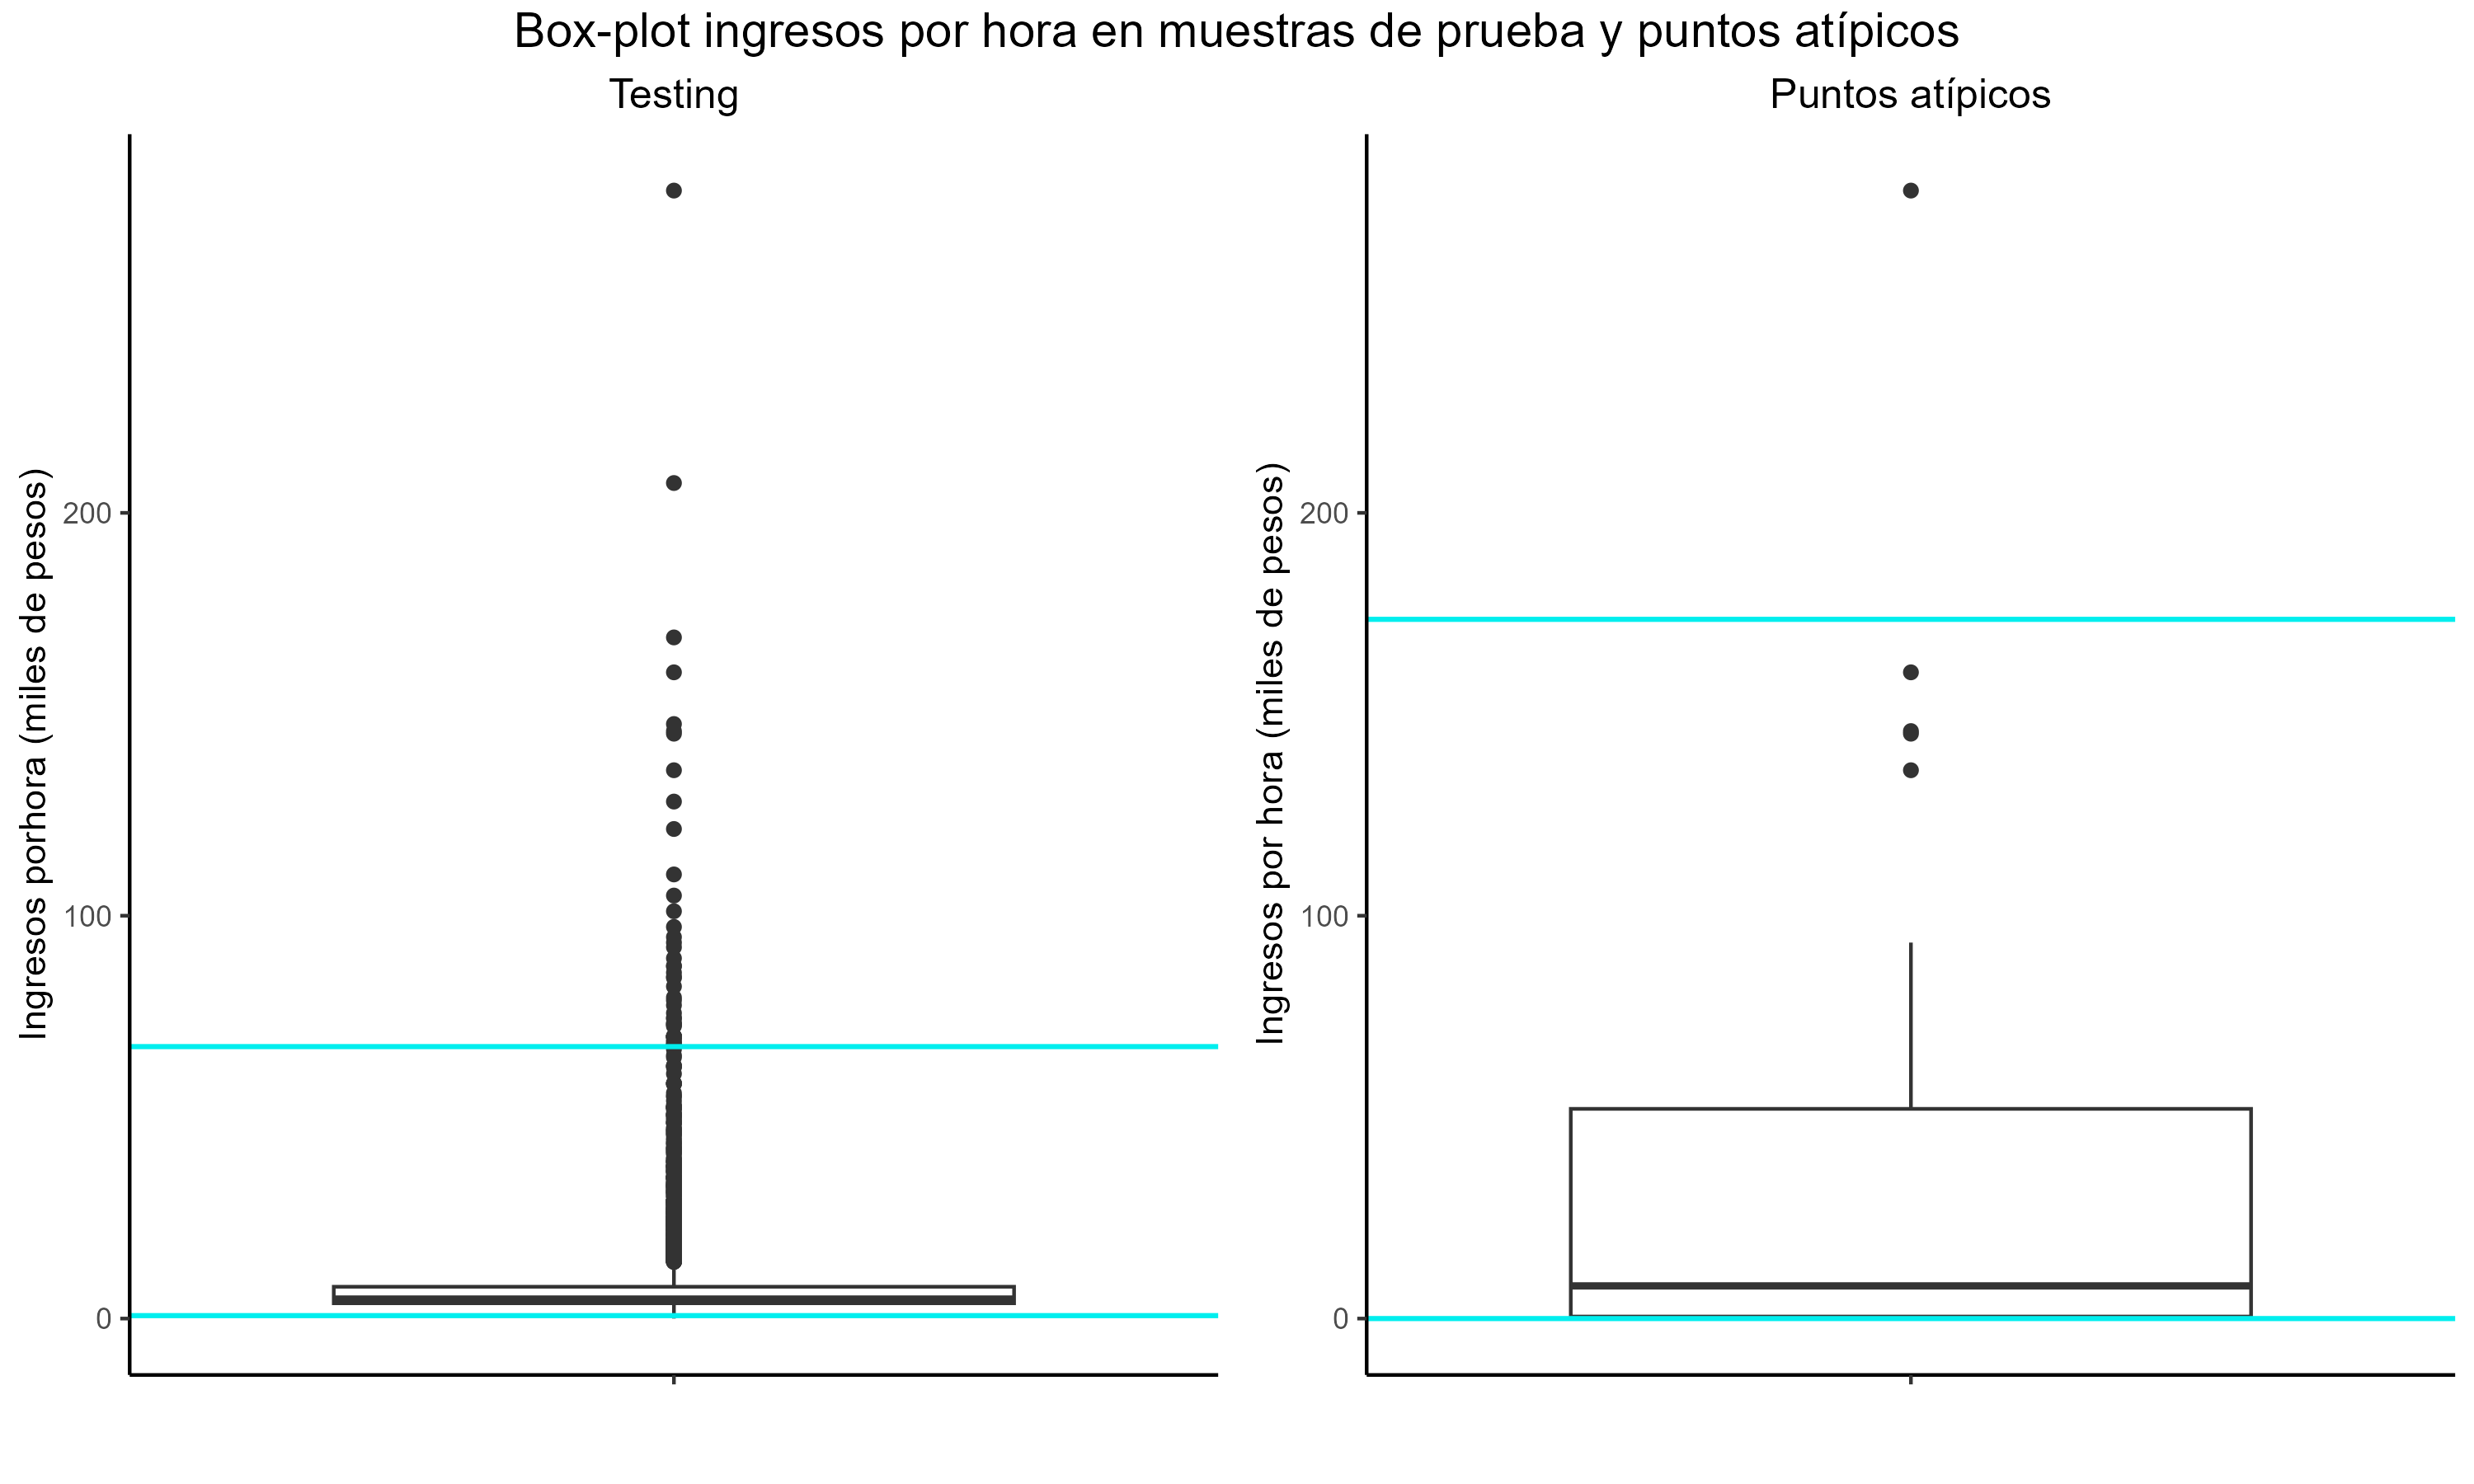
\includegraphics[width=0.8\linewidth]{bp_testing_outliers_p5.png}
    \caption{Box-plot ingresos por hora en muestras de prueba y puntos atípicos}
    \label{fig:bp_testing_outliers_p5}
     \begin{minipage}{15cm}
    \tiny Nota: \textit{Derecha:} muestra la distribución de los ingresos por hora en miles de pesos para la muestra de prueba en \textit{cross-validation}, \textit{Izquierda:} muestra la distribución de los ingresos por hora en miles de pesos para los datos atípicos ($outliers$) de la muestra de prueba en \textit{cross-validation}. Las líneas horizontales corresponden a los percentiles 99 (superior) y 1 (inferior) para cada variable
    \end{minipage}
\end{figure}

\begin{comment}
    {\color{red}\begin{itemize}
    \item[c.]En su discusión de los resultados, comente:
    \begin{itemize}
        \item Acerca del rendimiento general de los modelos.
        \item Acerca de la especificación con el menor error de predicción.
        \item Para la especificación con el menor error de predicción, explore aquellas observaciones que parecen \textit{miss the mark}. Para ello, {\color{teal}calcule los errores de predicción en la muestra de prueba y examine su distribución}. ¿Hay alguna observación en las colas de la distribución del error de predicción? ¿Son estos valores atípicos personas potenciales que la DIAN debería examinar, o son simplemente el producto de un modelo defectuoso?
    \end{itemize}
    \item[d.] LOOCV. Para los dos modelos con el menor error de predicción en la sección anterior, calcule el error de predicción utilizando la validación cruzada de dejar uno afuera (LOOCV). Compare los resultados del error de prueba con los obtenidos con el enfoque del conjunto de validación y explore los vínculos potenciales con la estadística de influencia. {\color{red}(Nota: al intentar realizar esta subsección, los cálculos pueden llevar mucho tiempo, según sus habilidades de codificación, ¡planifique en consecuencia!)}
\end{itemize}
\end{comment}

%%%%%%%%%%%%%%%%%%%%%%%%%%%%%%%%%%
% TABLA DIFERENCIA MEDIAS TESTING Y OUTLIERS TESTING
%%%%%%%%%%%%%%%%%%%%%%%%%%%%%%%%%%

\begin{table}[ht]
\centering
\caption{Diferencia de medias de variables entre muestras de prueba y outliers de la muestra de prueba}\label{diff_medias_CV}
\resizebox{\textwidth}{!}{ 
\begin{tabular}{lrrrrrrl}
  \hline
Variable & Mean\_testing & se\_test & Mean\_outliers & se\_out & Dif & p\_value & Significance \\ 
  \hline
formal & 59.6 & 0.7 & 36.7 & 5.1 & 23.0 & 0.0 & *** \\ 
  informal & 40.4 & 0.7 & 63.3 & 5.1 & -23.0 & 0.0 & *** \\ 
  Mujer & 47.1 & 0.8 & 55.6 & 5.2 & -8.5 & 0.1 &  \\ 
  Experiencia\_emp\_act & 5.1 & 0.3 & 2.2 & 1.6 & 2.9 & 0.3 &  \\ 
  Full\_time & 68.1 & 0.7 & 42.2 & 5.2 & 25.8 & 0.0 & *** \\ 
  Grupo\_etario\_Joven & 27.7 & 0.7 & 22.2 & 4.4 & 5.5 & 0.3 &  \\ 
  Grupo\_etario\_Adulto & 48.8 & 0.8 & 37.8 & 5.1 & 11.0 & 0.0 & *** \\ 
  Grupo\_etario\_Adulto\_m & 23.5 & 0.6 & 40.0 & 5.2 & -16.5 & 0.0 & *** \\ 
  Estrato\_1 & 10.9 & 0.5 & 8.9 & 3.0 & 2.0 & 0.7 &  \\ 
  Estrato\_2 & 43.3 & 0.7 & 30.0 & 4.8 & 13.3 & 0.0 & *** \\ 
  Estrato\_3 & 35.2 & 0.7 & 41.1 & 5.2 & -5.9 & 0.3 &  \\ 
  Estrato\_4 & 6.6 & 0.4 & 7.8 & 2.8 & -1.1 & 0.8 &  \\ 
  Estrato\_5 & 1.8 & 0.2 & 6.7 & 2.6 & -4.9 & 0.0 & *** \\ 
  Estrato\_6 & 2.2 & 0.2 & 5.6 & 2.4 & -3.3 & 0.1 &  \\ 
  Tamaño\_firma\_Micro & 50.2 & 0.8 & 76.7 & 4.5 & -26.5 & 0.0 & *** \\ 
  Tamaño\_firma\_Pequeña & 11.8 & 0.5 & 5.6 & 2.4 & 6.2 & 0.1 &  \\ 
  Tamaño\_firma\_Mediana\_grande & 38.0 & 0.7 & 17.8 & 4.0 & 20.3 & 0.0 & *** \\ 
  Ocupacion\_cat\_Obreros\_empleados & 62.7 & 0.7 & 23.3 & 4.5 & 39.4 & 0.0 & *** \\ 
  Ocupacion\_cat\_Emp\_domésticos & 3.7 & 0.3 & 3.3 & 1.9 & 0.3 & 1.0 &  \\ 
  Ocupacion\_cat\_Cuenta\_propia & 30.2 & 0.7 & 66.7 & 5.0 & -36.4 & 0.0 & *** \\ 
  Ocupacion\_cat\_Patron\_empleador & 3.3 & 0.3 & 6.7 & 2.6 & -3.3 & 0.1 &  \\ 
  Ocupacion\_cat\_Jornalero\_peon & 0.0 & 0.0 & 0.0 & 0.0 & 0.0 &  &  \\ 
  Ocupacion\_cat\_Otro & 0.1 & 0.0 & 0.0 & 0.0 & 0.1 & 1.0 &  \\ 
  y\_total\_m & 1,619,027.1 & 36,329.4 & 4,101,867.4 & 797,016.7 & -2,482,840.3 & 0.0 & *** \\ 
  y\_total\_m\_ha & 8,472.8 & 193.5 & 30,309.3 & 4,882.8 & -21,836.4 & 0.0 & *** \\ 
   \hline
    \hline
Observaciones & 4,427 & 90 &  &  &  &  &  \\ 
   \hline
\end{tabular}
}
\begin{minipage}{16cm}
\tiny Nota: Se realizó una prueba t con un nivel de significancia del 5\%. Para todas las variables, a excepción de $y\_total\_m$ y $y\_total\_m\_ha$ (ingreso mensual y por hora), la prueba de diferencia de medias se realizó con $prop.test$, en las dos restantes se usó $t.test$ de $R$.La muestra \textit{testing} corresponde al 30 \% de la muestra original en su versión final (descrita en la sección \ref{datos}) y la muestra \textit{outliers} proviene de la muestra \textit{testing} antes mencionada. 
\end{minipage}
\end{table}

En cuanto a la capacidad de predicción del modelo, se identifica una menor precisión en las colas de la distribución, lo que sugiere que el modelo tiene dificultades para capturar correctamente los valores extremos (los subestima) y parte de los valores medios los sobreestima (panel derecho figura \ref{fig:e_ajus_ob_CV_LOOV_m13_p5}). Asimismo, se presenta una situación similar con el modelo 12 (ver figura \ref{fig:e_ajus_ob_CV_LOOV_m12_p5}). Estos hallazgos se mantienen tanto para la estimación CV como LOOCV, lo que sugiere que no se trata de un error aleatorio sino de un patrón estructural en los datos. 
\bigbreak
Considerando las características incorporadas por el modelo para la predicción, la naturaleza de los datos (autoreporte), el ajuste relativamente bueno en los datos centrales, pero no hacia los extremos, y la descripción realizada sobre los ocupados en los valores extremos de los errores de predicción en la muestra de prueba, parece plausible que ese segmento de observaciones tenga un reporte distinto al real de los datos de ingreso. Es decir, hay varias razones por las cuales justificar una revisión fiscal por parte de la DIAN a esos ocupados. 
\bigbreak

\begin{figure}[ht]
    \centering
    \includegraphics[width=0.8\linewidth]{e_ajus_ob_CV_LOOV_m13_p5.png}
    \caption{Densidad de valores ajustados y observados (modelo 13) y errores de predicción para estimaciones CV y LOOCV}
    \label{fig:e_ajus_ob_CV_LOOV_m13_p5}
     \begin{minipage}{15cm}
    \tiny Nota: \textit{Derecha:} muestra la densidad de los valores observados en comparación con los ajustados del modelo 13 (mínimo MSE) estimados por \textit{cross-validation} así como \textit{Leave-One-Out cross validation}, \textit{Izquierda:} muestra los errores de predicción estimados a partir del modelo 13 (mínimo MSE) tanto por \textit{cross validation} así como \textit{Leave-One-Out cross validation}.
    \end{minipage}
\end{figure}

\bigbreak
Finalmente, se tienen los resultados de RMSE para \textit{cross-validation} y \textit{Leave-One-Out cross-validation}. En general, los resultados de LOOCV parecen ser ligeramente mejores que CV, lo que puede deberse a que LOOCV utiliza cada observación como un conjunto de prueba individual, permitiendo una evaluación más precisa del rendimiento del modelo. Sin embargo, la diferencia es pequeña, incluso, el LOOCV el mejor modelo es el 12, en CV es el 13 (cuadro \ref{RMSE_CV_LOOCV}). 


\begin{table}[ht]
\centering
\caption{Rendimiento predictivo en términos de RMSE: \textit{cross validation} 
 y \textit{Leave-One-Out cross validation (LOOCV)}}\label{RMSE_CV_LOOCV}
\begin{tabular}{lrr}
  \hline
Modelo & CV & LOOCV \\ 
  \hline
Modelo 12 & 0.57229 & 0.55821 \\ 
Modelo 13 & 0.57224 & 0.55872 \\ 
   \hline
\end{tabular}
   \begin{minipage}{0.8\textwidth}  
    \footnotesize \scriptsize { \textit{Notas:} Raíz del error de predicción cuadrático medio para los modelos especificados para \textit{cross validation} y \textit{Leave-One-Out cross validation}  (ver anexo \ref{modelos_LOOCV_anexo})}
    \end{minipage}
\end{table}

 El cambio marginal obsevado entre los errores de predicción obtenidos con CV y LOOCV podría estar relacionado con la estadística de influencia. LOOCV puede ser más robusto a esas observaciones ya que evalúa el modelo en cada punto de datos individualmente en iteraciones igual a las observaciones. Mientras que las observaciones con una alta influencia pueden afectar más las estimaciones  de CV, ya que depende de particiones más amplias del conjunto de datos.
\bigbreak
 
\begin{figure}[ht]
    \centering
    \includegraphics[width=0.8\linewidth]{e_ajus_ob_CV_LOOV_m12_p5.png}
    \caption{Densidad de valores ajustados y observados (modelo 12) y errores de predicción para estimaciones CV y LOOCV}
    \label{fig:e_ajus_ob_CV_LOOV_m12_p5}
     \begin{minipage}{15cm}
    \tiny Nota: \textit{Derecha:} muestra la densidad de los valores observados en comparación con los ajustados del modelo 12 (mínimo MSE) estimados por \textit{cross-validation} así como \textit{Leave-One-Out cross validation}, \textit{Izquierda:} muestra los errores de predicción estimados a partir del modelo 12 (mínimo MSE) tanto por \textit{cross validation} así como \textit{Leave-One-Out cross validation}.
    \end{minipage}
\end{figure}


%%%%%%%%%%%%%%%%%%%%%%%%%%%%%%%%%%%
%		  References				  %
%%%%%%%%%%%%%%%%%%%%%%%%%%%%%%%%%%%

\cleardoublepage
\singlespacing
\bibliography{References.bib}
\pagebreak

%%%%%%%%%%%%%%%%%%%%%%%%%%%%%%%%%%%
%		  TABLES				  %
%%%%%%%%%%%%%%%%%%%%%%%%%%%%%%%%%%%
\begin{comment}
\pagebreak
    
%\section*{Tables and Figures}


%\begin{figure}[H]
%\caption{US Map} \label{fig:robust}
%    \includegraphics[scale=0.75]{}   
% \flushleft
% Note: This figure shows ...
%\end{figure}

%%%%%%%%%%%%%%%%%%%%%%%%%%%%%%%%
%           APPENDIX	       %
%%%%%%%%%%%%%%%%%%%%%%%%%%%%%%%%
\pagebreak
\appendix
\renewcommand{\theequation}{\Alph{chapter}.\arabic{equation}}

\setcounter{figure}{0}
\setcounter{table}{0}
\makeatletter 
\renewcommand{\thefigure}{A.\@arabic\c@figure}
\renewcommand{\thetable}{A.\@arabic\c@table}
\end{comment}

\section{Apéndice}\label{sec:appendix_tables} 
\begin{figure}[H] 
    \centering
    \caption{}\label{boxplot_ing_mes}
    \includegraphics[width=0.7\textwidth]{Graphs/box_plot_m.png} 
\begin{minipage}{15cm}
\small Nota: las líneas horizontales corresponden a los percentiles 99 (superior) y 1 (inferior) para cada variable
\end{minipage}
\end{figure}


\subsection{Modelos especificados para CV y LOOCV:}\label{modelos_LOOCV_anexo}
\begin{align*}
\text{Modelo}_1: & \quad \log(\text{y\_total\_m\_ha}) = \beta_0 + \beta_1 \text{poly}(\text{age}, 2) + \epsilon \\
\\
\text{Modelo}_2: & \quad \log(\text{y\_total\_m\_ha}) = \beta_0 + \beta_1 \text{Mujer} + \beta_2 \text{poly}(\text{age}, 2) + \beta_3 I(\text{Max\_nivel\_educacion}) + \\ & \quad 
\beta_4 \text{poly}(\text{Experiencia\_emp\_act}, 2) + \beta_5 I(\text{Tamaño\_firma\_c3}) + \\ & \quad 
\beta_6 \text{Full\_time} + \beta_7 \text{formal} +  \beta_8 I(\text{Oficio\_cat}) +  \epsilon \\
\\
\text{Modelo}_3: & \quad \log(\text{y\_total\_m\_ha}) = \beta_0 + \beta_1 \text{Mujer} + \beta_2 \text{poly}(\text{age}, 2) + \beta_3 I(\text{Max\_nivel\_educacion}) + \\ & \quad 
\beta_4 \text{poly}(\text{Experiencia\_emp\_act}, 2) + \beta_5 I(\text{Tamaño\_firma\_c5}) + \\ & \quad 
\beta_6 \text{Full\_time} + \beta_7 \text{formal} + \beta_8 I(\text{Oficio\_cat})+ \epsilon \\
\\
\text{Modelo}_4: & \quad \log(\text{y\_total\_m\_ha}) = \beta_0 + \beta_1 \text{Mujer} + \beta_2 \text{poly}(\text{age}, 3):\text{Mujer} + \beta_3 \text{poly}(\text{age}, 3) \\
& \quad + \beta_4 I(\text{Max\_nivel\_educacion2}) + \beta_5 \text{poly}(\text{age}, 3) : I(\text{Max\_nivel\_educacion2}) + \\
& \quad \beta_6 \text{poly}(\text{Experiencia\_emp\_act}, 3) + \beta_7 I(\text{Tamaño\_firma\_c5}) + \\
& \quad \beta_8 \text{Full\_time} + \beta_9 \text{formal} + \beta_8 I(\text{Oficio\_cat}) + \epsilon \\
\\
\text{Modelo}_5: & \quad \log(\text{y\_total\_m\_ha}) = \beta_0 + \beta_1 \text{Mujer} + \beta_2 \text{poly}(\text{age}, 2) + \beta_3 I(\text{Max\_nivel\_educacion}) + \\ & \quad 
\beta_4 \text{poly}(\text{Experiencia\_emp\_act}, 2) + \beta_5 I(\text{Tamaño\_firma\_c5}) + \\ & \quad 
\beta_6 \text{Full\_time} + \beta_7 \text{formal} + \\ & \quad 
\beta_8 I(\text{children\_6years}) + \beta_9 I(\text{Oficio\_cat}) + \epsilon \\
\\
\text{Modelo}_6: & \quad \log(\text{y\_total\_m\_ha}) = \beta_0 + \beta_1 \text{Mujer} + \beta_2 \text{poly}(\text{age}, 3):\text{Mujer} + \beta_3 \text{poly}(\text{age}, 3) \\
& \quad + \beta_4 I(\text{Max\_nivel\_educacion2}) + \beta_5 \text{poly}(\text{age}, 3) : I(\text{Max\_nivel\_educacion2}) + \\
& \quad \beta_6 \text{poly}(\text{Experiencia\_emp\_act}, 3) + \beta_7 I(\text{Tamaño\_firma\_c5}) + \\
& \quad \beta_8 \text{Full\_time} + \beta_9 \text{formal} + \\ & \quad \beta_{10} I(\text{children\_6years}) + \beta_{11} I(\text{Oficio\_cat}) + \epsilon \\
\\
\text{Modelo}_7: & \quad \log(\text{y\_total\_m\_ha}) = \beta_0 + \beta_1 \text{Mujer} + \beta_2 \text{poly}(\text{age}, 4) : \text{Mujer} + \beta_3 \text{poly}(\text{age}, 4) \\
& \quad + \beta_4 I(\text{Max\_nivel\_educacion2}) + \beta_5 \text{poly}(\text{age}, 4) : I(\text{Max\_nivel\_educacion2}) + \\
& \quad \beta_6 \text{poly}(\text{Experiencia\_emp\_act}, 4)  + \beta_7 I(\text{Tamaño\_firma\_c5}) + \\
& \quad \beta_8 \text{Full\_time} + \beta_9 \text{formal} + \beta_{10} I(\text{Oficio\_cat})+\\ & \quad \beta_{11} I(\text{children\_6years}) + \epsilon \\
\\
\text{Modelo}_8: & \quad \log(\text{y\_total\_m\_ha}) = \beta_0 + \beta_1 \text{Mujer} + \beta_2 \text{poly}(\text{age}, 3) : \text{Mujer} + \beta_3 \text{poly}(\text{age}, 3) \\
& \quad + \beta_4 I(\text{Max\_nivel\_educacion2}) + \beta_5 \text{poly}(\text{age}, 3) : I(\text{Max\_nivel\_educacion2}) + \\
& \quad \beta_6 \text{poly}(\text{Experiencia\_emp\_act}, 3) + \beta_7 I(\text{Tamaño\_firma\_c5}) +  \\
& \quad \beta_8 \text{Full\_time} + \beta_9 \text{formal} +  \beta_{10} I(\text{Oficio\_cat}) + \\
& \beta_{11} \quad I(\text{children\_6years}) + \beta_{12} I(\text{children\_6years}):Mujer + \epsilon \\
\\
\text{Modelo}_9: & \quad \log(\text{y\_total\_m\_ha}) = \beta_0 + \beta_1 \text{Mujer} + \beta_2 \text{poly}(\text{age}, 4) : \text{Mujer} + \beta_3 \text{poly}(\text{age}, 4) \\
& \quad + \beta_4 I(\text{Max\_nivel\_educacion2}) + \beta_5 \text{poly}(\text{age}, 4) : I(\text{Max\_nivel\_educacion2}) +  \\
& \quad \beta_6 \text{poly}(\text{Experiencia\_emp\_act}, 4) + \beta_7 I(\text{Tamaño\_firma\_c5}) +  \\
& \quad \beta_8 \text{Full\_time} + \beta_9 \text{formal} + \beta_{10} I(\text{Oficio\_cat}) + \\
& \quad \beta_{11} I(\text{children\_6years}) + \beta_{12} I(\text{children\_6years}):Mujer + \epsilon \\
\\
\text{Modelo}_{10}: & \quad \log(\text{y\_total\_m\_ha}) = \beta_0 + \beta_1 \text{Mujer} + \beta_2 \text{poly}(\text{age}, 3) : \text{Mujer} + \beta_3 \text{poly}(\text{age}, 3) \\
& \quad + \beta_4 I(\text{Max\_nivel\_educacion2}) + \beta_5 \text{poly}(\text{age}, 3) : I(\text{Max\_nivel\_educacion2}) + \\
& \quad \beta_6 \text{poly}(\text{Experiencia\_emp\_act}, 3) + \beta_7 I(\text{Tamaño\_firma\_c5}) +  \\
& \quad \beta_8 \text{Full\_time} + \beta_9 \text{formal} +  \\
& \quad \beta_{10} I(\text{Ocupacion}) + \beta_{11} I(\text{Oficio\_cat}) + \\ & \quad \beta_{12} I(\text{children\_6years}) + \beta_{13} I(\text{children\_6years}):Mujer + \epsilon \\
\\
\text{Modelo}_{11}: & \quad \log(\text{y\_total\_m\_ha}) = \beta_0 + \beta_1 \text{Mujer} + \beta_2 \text{poly}(\text{age}, 4) : \text{Mujer} + \beta_3 \text{poly}(\text{age}, 4) \\
& \quad + \beta_4 I(\text{Max\_nivel\_educacion2}) + \beta_5 \text{poly}(\text{age}, 4) : I(\text{Max\_nivel\_educacion2}) +  \\
& \quad \beta_6 \text{poly}(\text{Experiencia\_emp\_act}, 4) + \beta_7 I(\text{Tamaño\_firma\_c5}) +  \\
& \quad \beta_8 \text{Full\_time} + \beta_9 \text{formal} +  \\
& \quad \beta_{10} I(\text{Ocupacion}) + \beta_{11} I(\text{oficio}) + \\ & \quad \beta_{12} I(\text{children\_6years}) + \beta_{13} I(\text{children\_6years}):Mujer + \epsilon \\
\\
\text{Modelo}_{12}: & \quad \log(\text{y\_total\_m\_ha}) = \beta_0 + \beta_1 \text{Mujer} + \beta_2 \text{poly}(\text{age}, 3) : \text{Mujer} + \beta_3 \text{poly}(\text{age}, 3) \\
& \quad + \beta_4 I(\text{Max\_nivel\_educacion2}) + \beta_5 \text{poly}(\text{age}, 3) : I(\text{Max\_nivel\_educacion2}) +  \\
& \quad \beta_6 \text{poly}(\text{Experiencia\_emp\_act}, 3) + \beta_7 I(\text{Tamaño\_firma\_c5}) +  \\
& \quad \beta_8 \text{Full\_time} + \beta_9 \text{formal} +  \\
& \quad \beta_{10} I(\text{Ocupacion}) + \beta_{11} I(\text{oficio}) + \\
& \quad \beta_{12} I(\text{Cot\_pension}) + \beta_{13} \text{Jefe\_hogar} + \beta_{14} I(\text{Estrato}) + \\ & \quad \beta_{15} I(\text{children\_6years}) + \beta_{16} I(\text{children\_6years}):Mujer + \epsilon \\
\\
\text{Modelo}_{13}: & \quad \log(\text{y\_total\_m\_ha}) = \beta_0 + \beta_1 \text{Mujer} + \beta_2 \text{poly}(\text{age}, 4) : \text{Mujer} + \beta_3 \text{poly}(\text{age}, 4) \\
& \quad + \beta_4 I(\text{Max\_nivel\_educacion2}) + \beta_5 \text{poly}(\text{age}, 4) : I(\text{Max\_nivel\_educacion2}) +  \\
& \quad \beta_6 \text{poly}(\text{Experiencia\_emp\_act}, 4) + \beta_7 I(\text{Tamaño\_firma\_c5}) +  \\
& \quad \beta_8 \text{Full\_time} + \beta_9 \text{formal} +  \\
& \quad \beta_{10} I(\text{Ocupacion}) + \beta_{11} I(\text{oficio}) +  \\
& \quad \beta_{12} I(\text{Cot\_pension}) + \beta_{13} \text{Jefe\_hogar} + \beta_{14} I(\text{Estrato}) + \\ & \quad \beta_{15} I(\text{children\_6years}) + \beta_{16} I(\text{children\_6years}):Mujer + \epsilon \\
\\
\text{Modelo}_{14}: & \quad \log(\text{y\_total\_m\_ha}) = \beta_0 + \beta_1 \text{Mujer} + \beta_2 \text{poly}(\text{age}, 6) : \text{Mujer} + \beta_3 \text{poly}(\text{age}, 6) \\
& \quad + \beta_4 I(\text{Max\_nivel\_educacion2}) + \beta_5 \text{poly}(\text{age}, 6) : I(\text{Max\_nivel\_educacion2}) +  \\
& \quad \beta_6 \text{poly}(\text{Experiencia\_emp\_act}, 6) + \beta_7 I(\text{Tamaño\_firma\_c5}) +  \\
& \quad \beta_8 \text{Full\_time} + \beta_9 \text{formal} +  \\
& \quad \beta_{10} I(\text{Ocupacion}) + \beta_{11} I(\text{oficio}) +  \\
& \quad \beta_{12} I(\text{Cot\_pension}) + \beta_{13} \text{Jefe\_hogar} + \beta_{14} I(\text{Estrato}) + \\ & \quad \beta_{15} I(\text{children\_6years}) + \beta_{16}I(\text{children\_6years}):Mujer + \epsilon \\
\end{align*}


\end{document}
